\documentclass[fleqn]{article}

\usepackage{polski}
\usepackage[utf8]{inputenc}
\usepackage[polish]{babel}
\usepackage{parskip}
\usepackage{icomma}
\usepackage[a4paper,includeheadfoot,margin=1.27cm]{geometry}
\usepackage{float}
\usepackage{graphicx}
\usepackage{amsmath}
\usepackage[hypcap=true]{subcaption}
\usepackage{xcolor}
\usepackage{transparent}
\usepackage{listings}
\usepackage[colorlinks=true, linkcolor=blue, pdfborder={0 0 0}]{hyperref}

\renewcommand\thesection{\arabic{section}.}
\renewcommand\thesubsection{\alph{subsection})}
\renewcommand\thesubsubsection{}
\newcommand\square[1]{
	\fcolorbox{black}{#1}{\rule{0pt}{6pt}\rule{6pt}{0pt}}
}

\brokenpenalty=1000
\clubpenalty=1000
\widowpenalty=1000

\title{\textbf{STP} \\ \large Projekt II - Zadanie 2.39}
\author{Marcin Skrzypkowski \\ nr albumu 283419}

\begin{document}

\maketitle

\setcounter{page}{0}
\thispagestyle{empty}

\pagebreak
\setcounter{page}{1}


\tableofcontents
\pagebreak


\begin{center}

	Obiekt regulacji jest opisany poniższą transmitancją

	\Large{\textbf{G($s$)=}$\frac{K_oe^{-T_os}}{(T_1s+1)(T_2s+1)}$}
\end{center}

\begin{table}[H]
	\centering
	\label{my-label}
	\begin{tabular}{|l|l|l|l|l|}\hline
		% &K & T_1 & T_2 &   \alpha_1 & \alpha_2 & \alpha_3 & \alpha_4 \\ \hline
		% &$5.5$ & $7$ & $7$ &$-0.12$ & $0.4$ & $0.25$ & $0.2$\\ \hline
		$K_o$ & $T_o$ &$T_1$ &  $T_2$   \\ \hline
		$4.5$ & $5$ & $1.87$ &$5.31$\\ \hline
	\end{tabular}
	\caption{Wartości parametrów obiektu regulacji}
\end{table}

\section{Wyznaczenie transmitancji dyskretnej}

W celu wyznaczenia transmitancji dyskretnej obiektu wykorzystana została funkccja \textit{c2d}. Po ustaleniu okresu próbkowania na $0.5$s i wykorzystaniu ekstrapolatora zerowego rzędu porównano odpowiedzi skokowe obiektu ciągłego i dyskretnego. Ekstrapolator spełnia równanie:
{\Large
\begin{equation}
	G(z)=\frac{1-z^{-1}}{z}\mathcal{Z}\bigg\{\frac{G(s)}{s}\bigg\}
\end{equation}

}

Transmitancja dyskretna ma postać
{\Large
\begin{equation}
	G(z)=z^{-10}\frac{0.05029z+0.04458}{z^2-1.676z+0.6966}
\end{equation}
}

Poniższe wyniki potwierdzają prawidłowe wyznaczenie obiektu dyskretnego, gdyż obie odpowiedzi się pokrywają.

\begin{figure}[H]
	\centering
	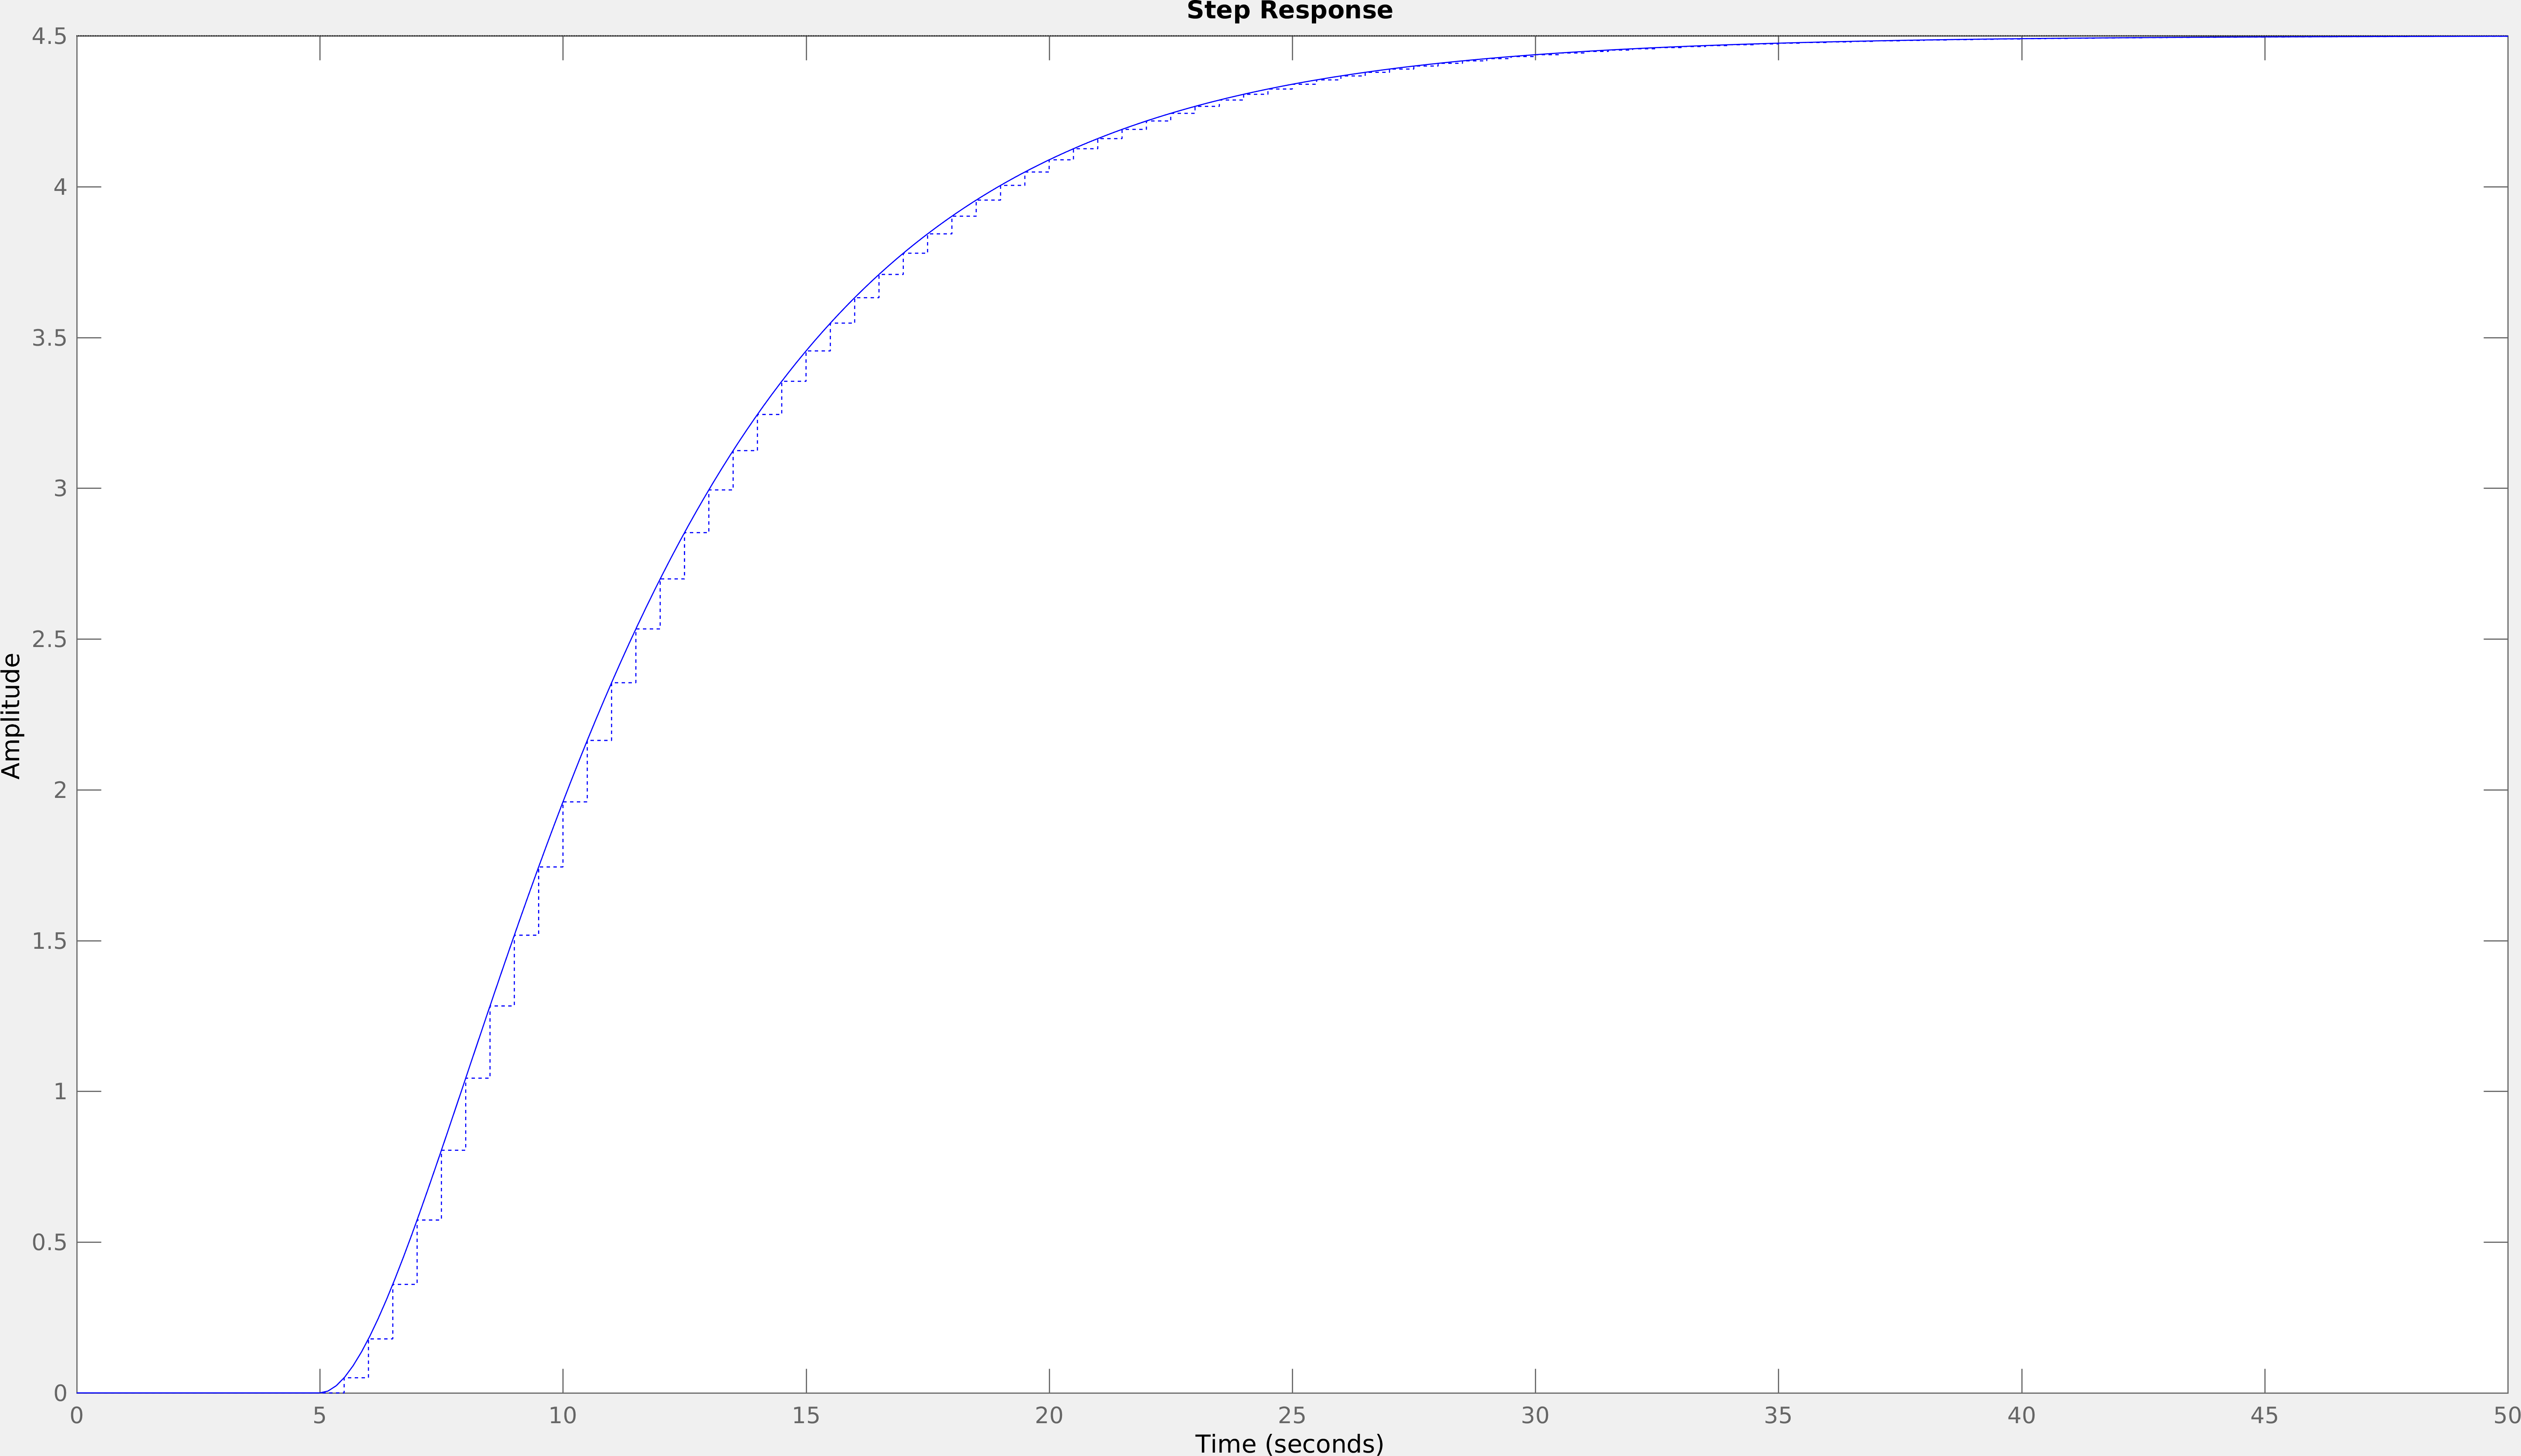
\includegraphics[width=\textwidth]{scripts/odpowiedzskok.png}
	\caption{odpowiedź skokowa obiektu ciągłego i dyskretnego}
	\label{}
\end{figure}

 Ekstrapolator zerowego rzędu nie jest przybliżeniem obiektu regulacji jak to ma miejsce w przypadku emulacji przykładowo wzorem Eulera, lecz pozwala dobierać regulator cyfrowy bezpośrednio na niezaokrąglonej odpowiedzi obiektu.

 Następnie wyznaczono wartości wzmocnienia statycznego trnamsitancji ciągłej i dyskretnej korzystając z następujących wzorów:
{\Large
\begin{equation}
	K_s=\lim_{s\to 0}sX(s)= 4.5
\end{equation}
\begin{equation}
	K_z=\lim_{z\to 1}(1-z^{-1})Y(z)\approx 4.6053
\end{equation}
}

odpowiedzi skokowe obu transmitancji mają praktycznie takie same wartości z dokłądnością do współczynników wyznaczonych przez funkcję \textit{c2d}.

\section{Równanie różnicowe}

Równanie różnicowe postaci
{\Large
\begin{equation}
		y(k)=\sum\limits_{i=1}^{n}b_iy(k-i)+\sum\limits_{i=1}^mc_iu(k-i)
\end{equation}
}

Wyznacza się przez przekształcenie postaci transmitancji dyskretnej, która jest równa stosunkowi wyjścia obiektu do jego sterowania

{\Large
\begin{equation}
	\frac{Y(z)}{X(z)}=\frac{c_mz^m + c_{m-1}z^{m-1}+\dots+c_1z+c_0}{z^n+b_{n-1}z^{n-1}+\dots+b_1z+b_0}
\end{equation}}

Po przekształceniu równanie ma postać

{\Large
\begin{equation}
	y(k)=0.05029u(k-11)+0.04458u(k-12)+1.676y(k-1)-0.6966y(k-2)
\end{equation}
}
\pagebreak

\section{Ciągły regulator PID}

Ciągły równoległy regulator PID opisany jest rónwaniem transmitacji

{\Large
\begin{equation}
	U(s)=K_r(1+\frac{1}{T_is}+T_ds)E(s)
\end{equation}
}

W celu dobrania nastaw wykorzystano metodę Zieglera-Nicholsa. Algorytm wygląda następująco:
\begin{itemize}
	\item wyłączyć człony całkujący i różniczkujący regulatora
	\item dobrać możliwe dużą wartość współczynnika członu proporcjonalnego ($K_k$), aby dotrzeć do granicy stabilności obiektu przy odpowiedzi skokowej
	\item zbadać okres oscylacji wyznaczonych w poprzednim punkcie ($T_k$)
	\item obliczyć nastawy regulatora $K_r=0.6K_k, T_i=0.5T_k, T_d=0.12T_k$
\end{itemize}

Mimo wielu prób nie udało się osiągnąć bardziej satysfakcjonującego wyniku regulacji niż przy nastawach wyznaczonych metodą Zieglera-Nicholsa. Poniżej znajduje się wykres kilku iteracji regulacji dla różnych wartości $T_i$ oraz $T_d$

\begin{figure}[H]
	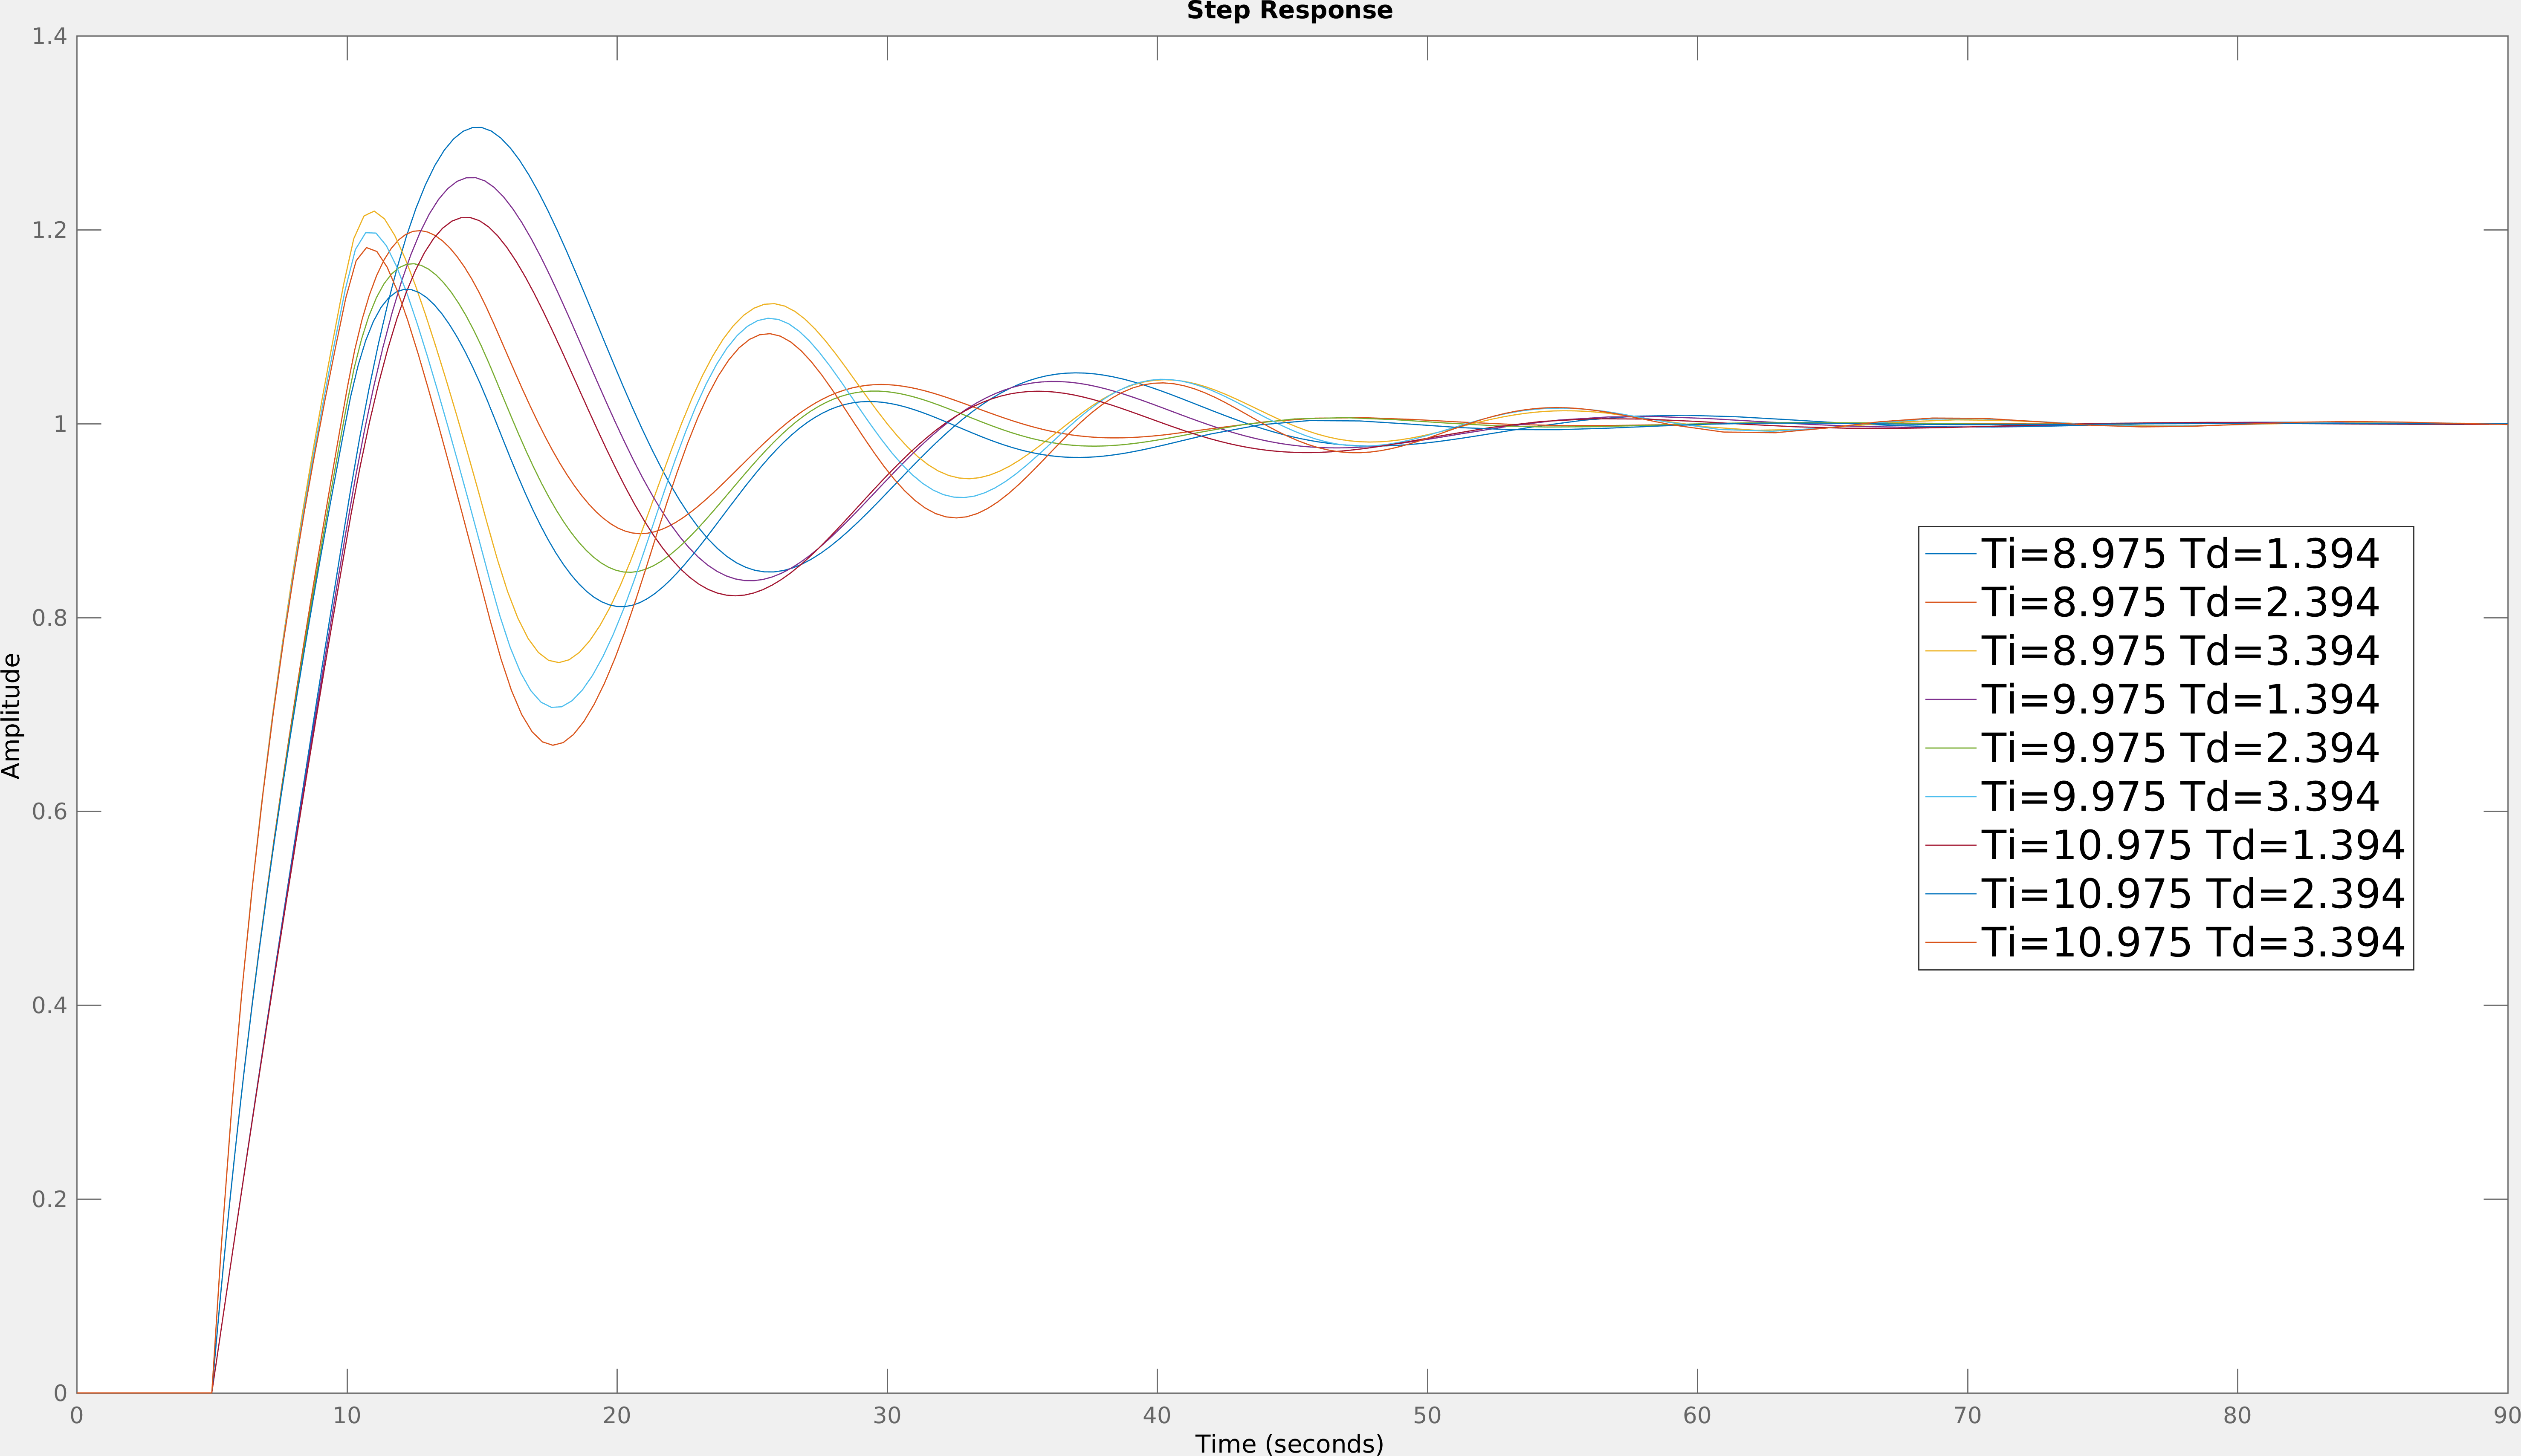
\includegraphics[width=\textwidth]{scripts/odpowiedzskokZN.png}
	\caption{Próba dostrojenia regulatora PID, $K_k = 0.5012$}
\end{figure}

Obliczone wartości współczynników po algorytmie Zieglera-Nicholsa:
\begin{itemize}
	\item $K_r = 0.5019$
	\item $T_i = 9.975$
	\item $T_d = 2.394$
\end{itemize}
\pagebreak
Po eksperymentowaniu również z wartością współczynnika proporcjonalnego udało się otrzymać następujące wyniki

\begin{figure}[H]
	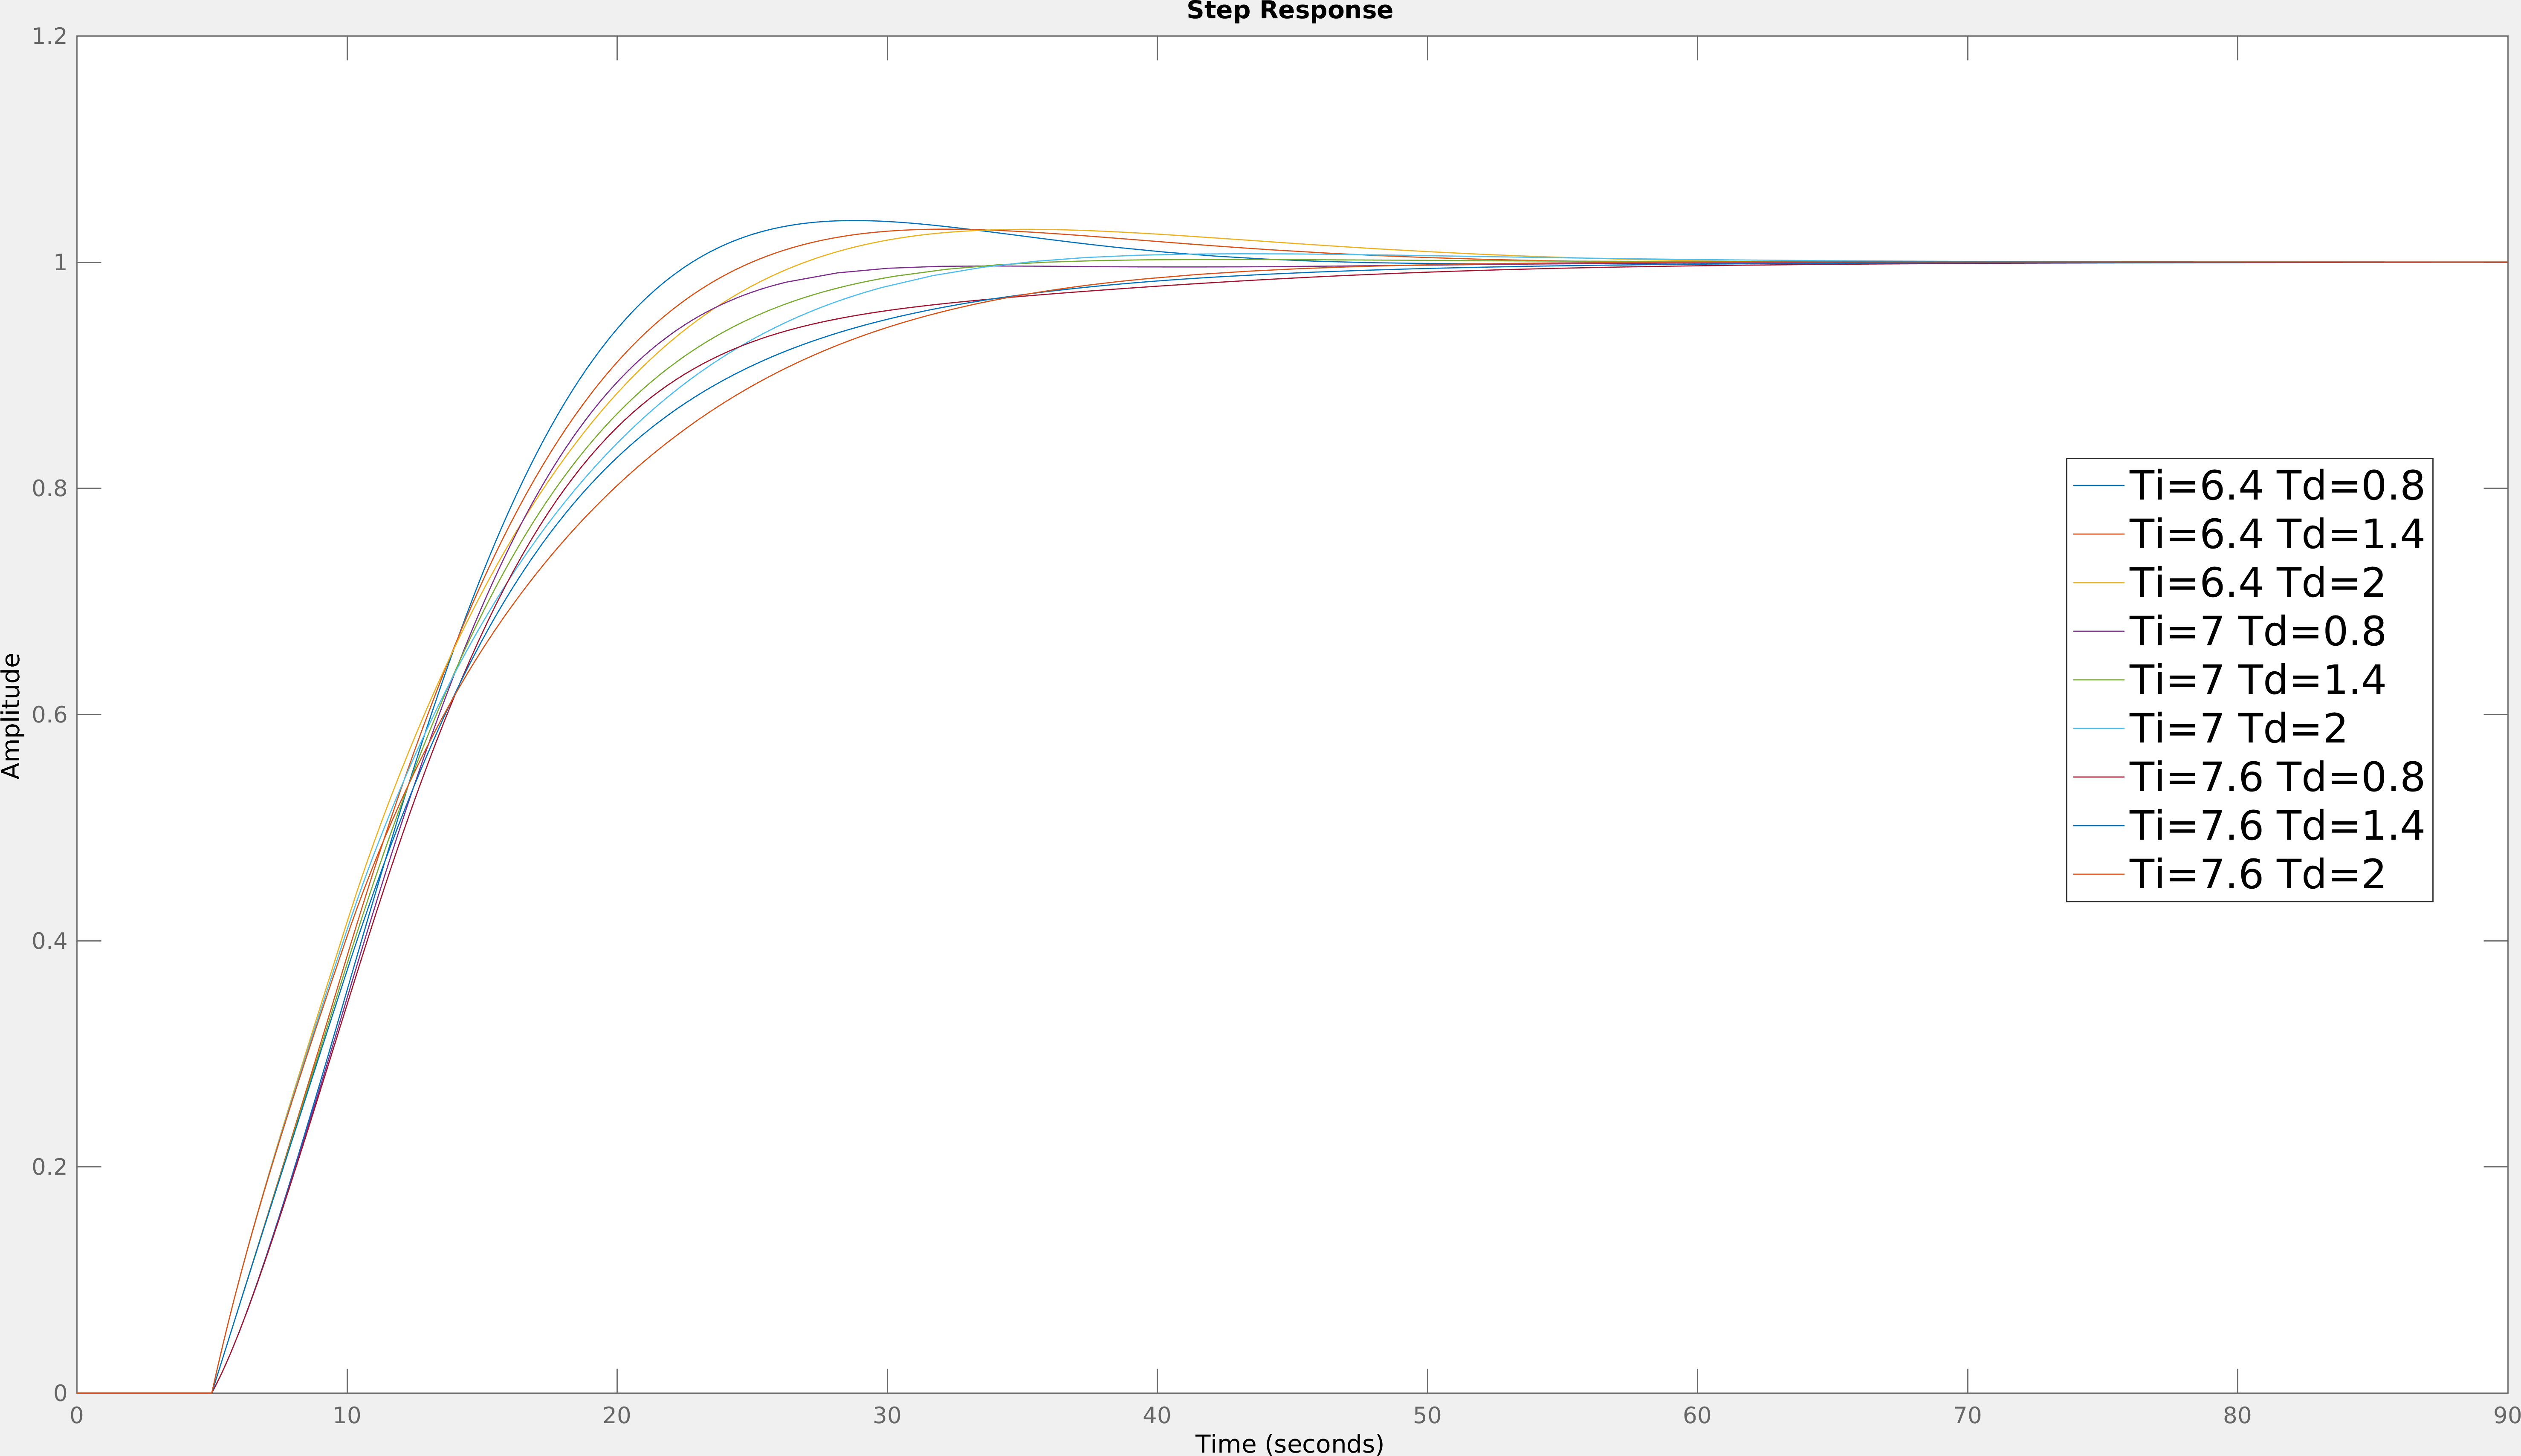
\includegraphics[width=\textwidth]{scripts/odpowiedzskokM.png}
	\caption{Odpowiedź skokowa po zmniejszeniu współczynnika $K_r$ do 0.2}
\end{figure}

Najlepsze nastawy, jakie udało się uzyskać, mają wartości
\begin{itemize}
	\item $K_r = 0.2$
	\item $T_i = 7$
	\item $T_d = 0.8$
\end{itemize}

Przemawiają za nimi brak oscylacji oraz zdecydowanie krótszy czas regulacji.

Następne doświadczenia będą przeprowadzane w dwóch przypadkach, dla nastaw wyznaczonych metodą Z-N oraz najlepszych znalezionych.

\section{Regulatory dyskretne}

Następnym zadaniem było wyznaczenie nastaw regulatora cyfrowego. Ma on postać
{\Large
\begin{equation}
	U(k)=r_2E(k-2)+r_1E(k-1)+r_0E(k)
\end{equation}
}

gdzie
{\Large
\begin{equation}
	r_0=K_r(1+\frac{T_p}{2T_i}+\frac{T_d}{T_p})\\
	r_1=K_r(\frac{T_p}{2T_i}-2*\frac{2T_d}{T_p}-1)\\
	r_2=K_r\frac{T_d}{T_p}
\end{equation}
}
$T_p$ to okres próbkowania, w tym przypadku wynosi on $0.5$s.
\pagebreak
\subsection{Nastawy Zieglera-Nicholsa}

Po podstawieniu wyznaczonych wcześniej wartości wspołczynników otrzymano następujące wartości parametrów regulatora cyfrowego
\begin{itemize}
	\item $r_0 = 1.7481$
	\item $r_1 = -3.1729$
	\item $r_2 = 1.4398$
\end{itemize}


\subsection{Nastawy poprawione}
Poniżej znajdują się wartości współczynników obliczonych na podstawie poprawionego regulatora ciągłego.
\begin{itemize}
	\item $r_0 = 0.5271$
	\item $r_1 = -0.8329$
	\item $r_2 = 0.32$
\end{itemize}

\subsection{Porównanie}
\begin{figure}[H]
	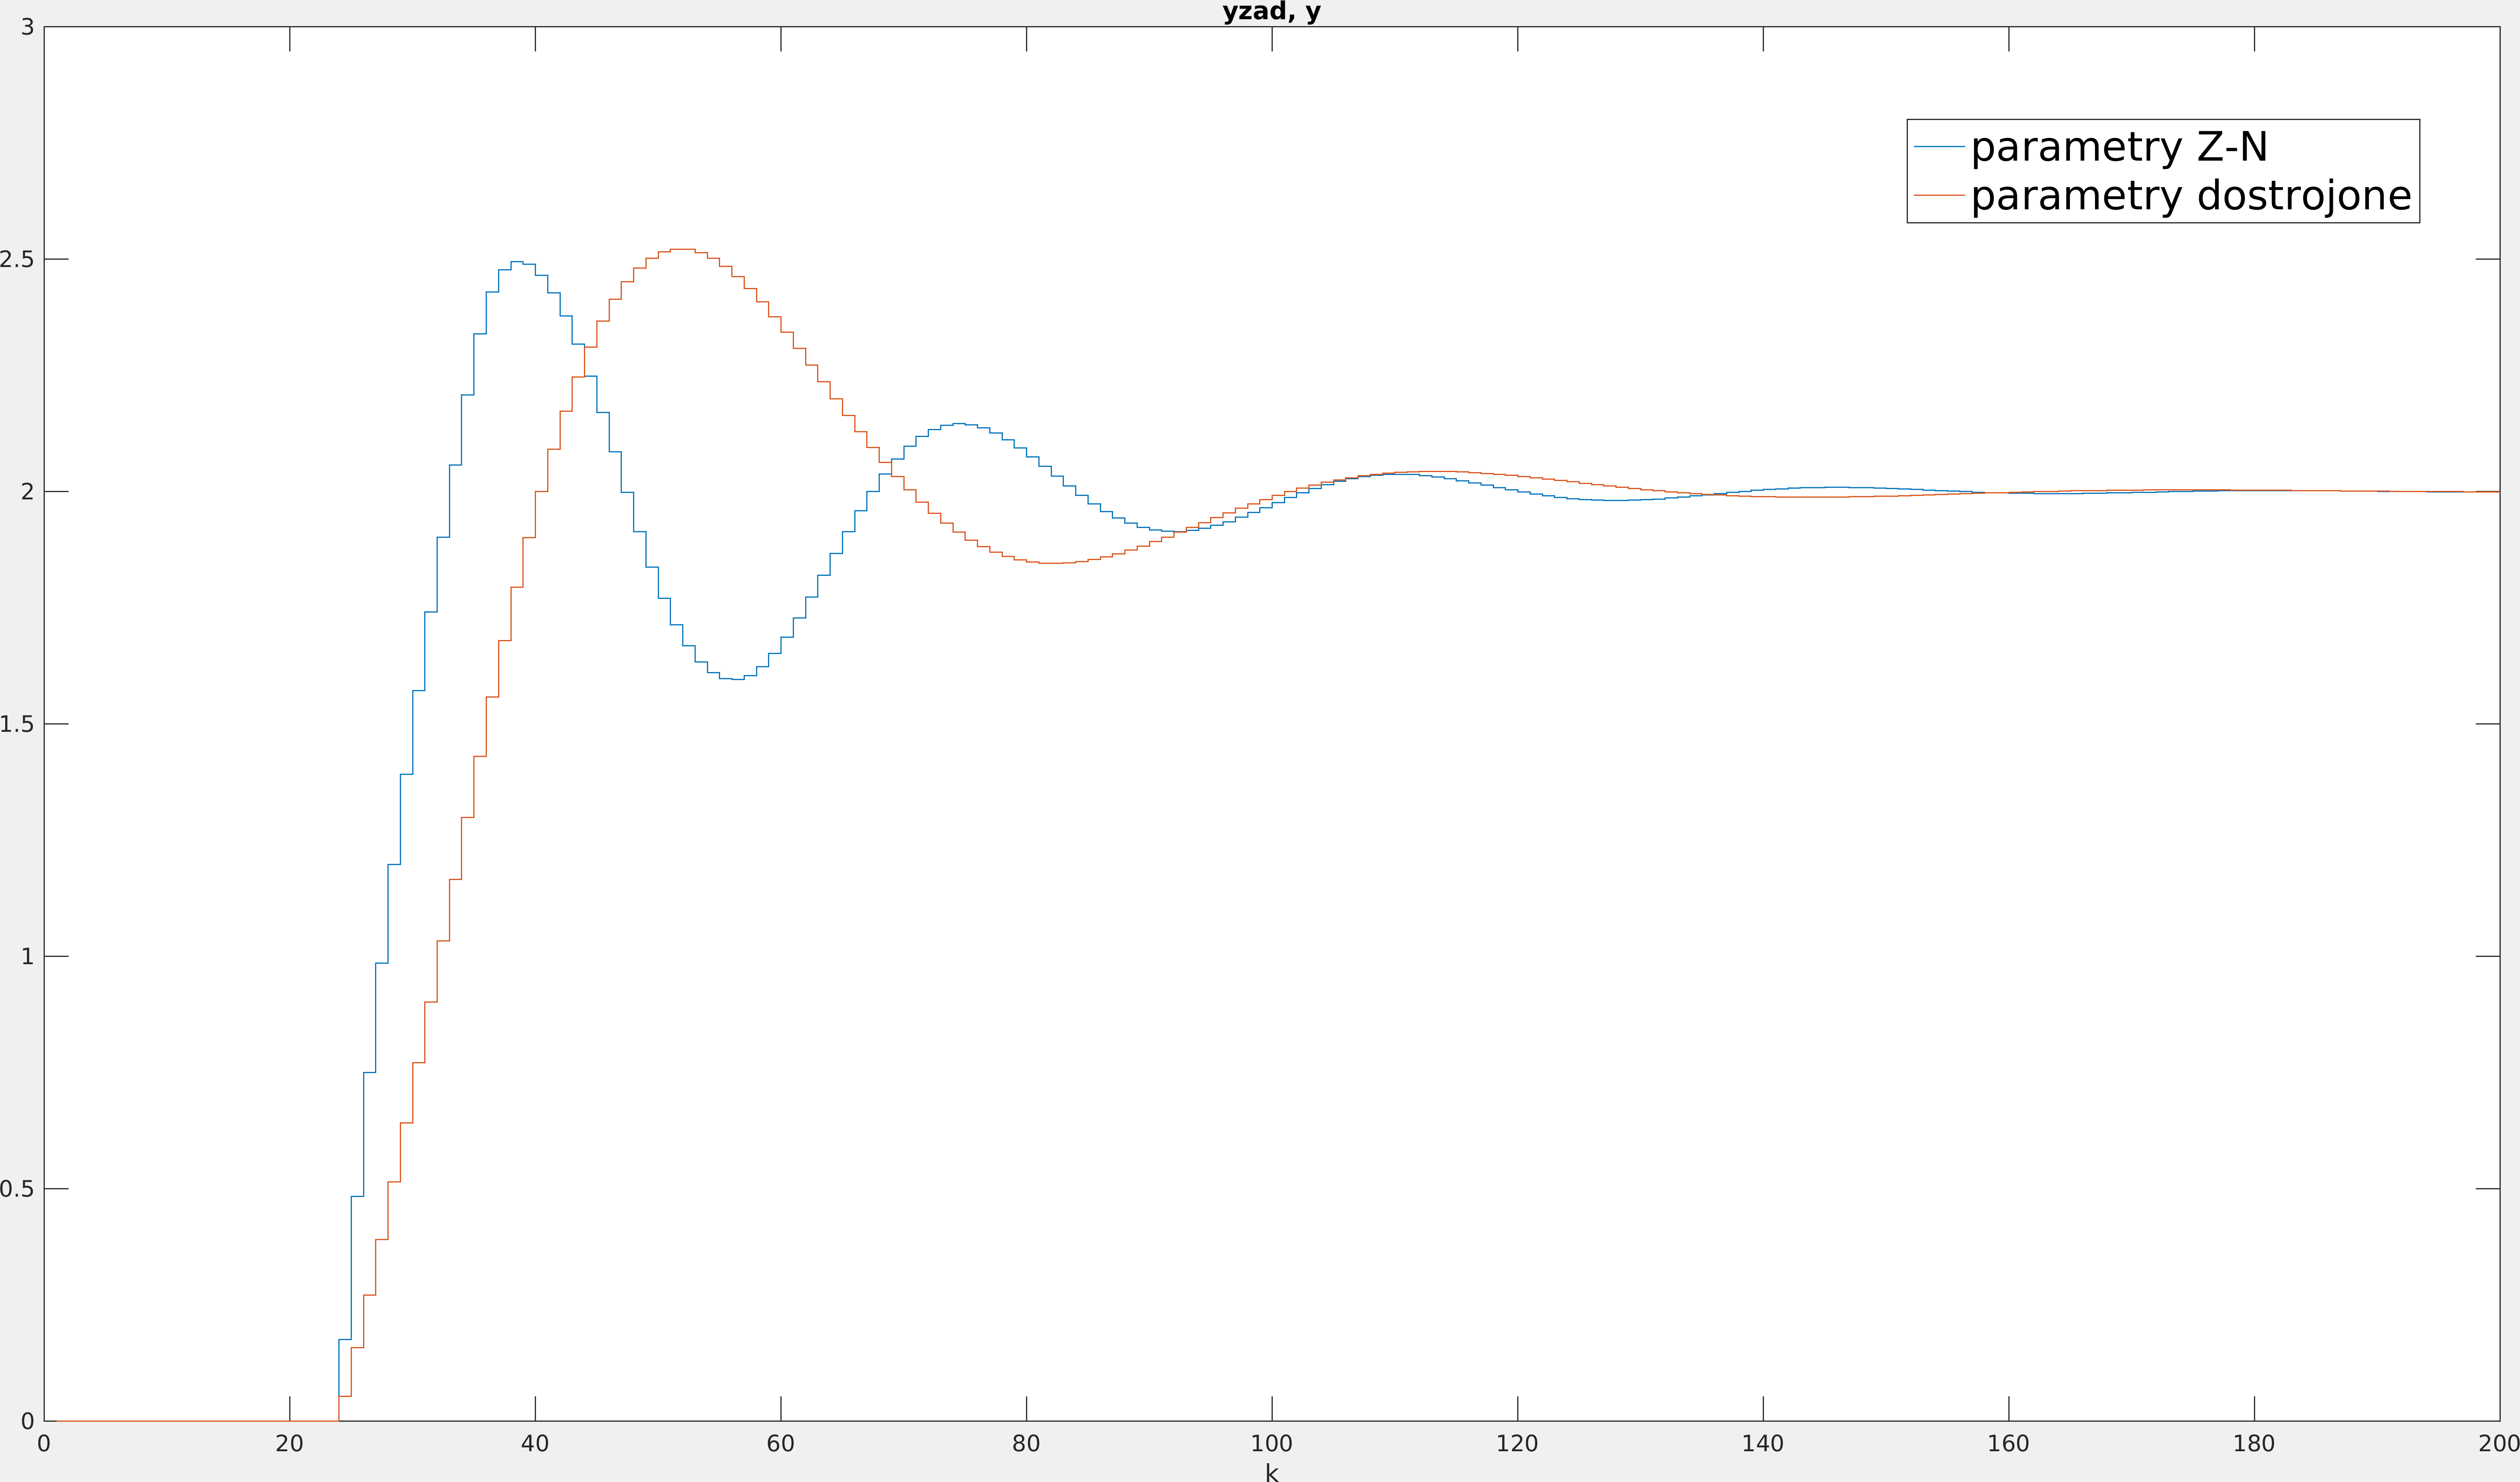
\includegraphics[width=\textwidth]{scripts/dyskretwyj.png}
	\caption{wyjście obiektu regulacji cyfrowej}
\end{figure}

\begin{figure}[H]
	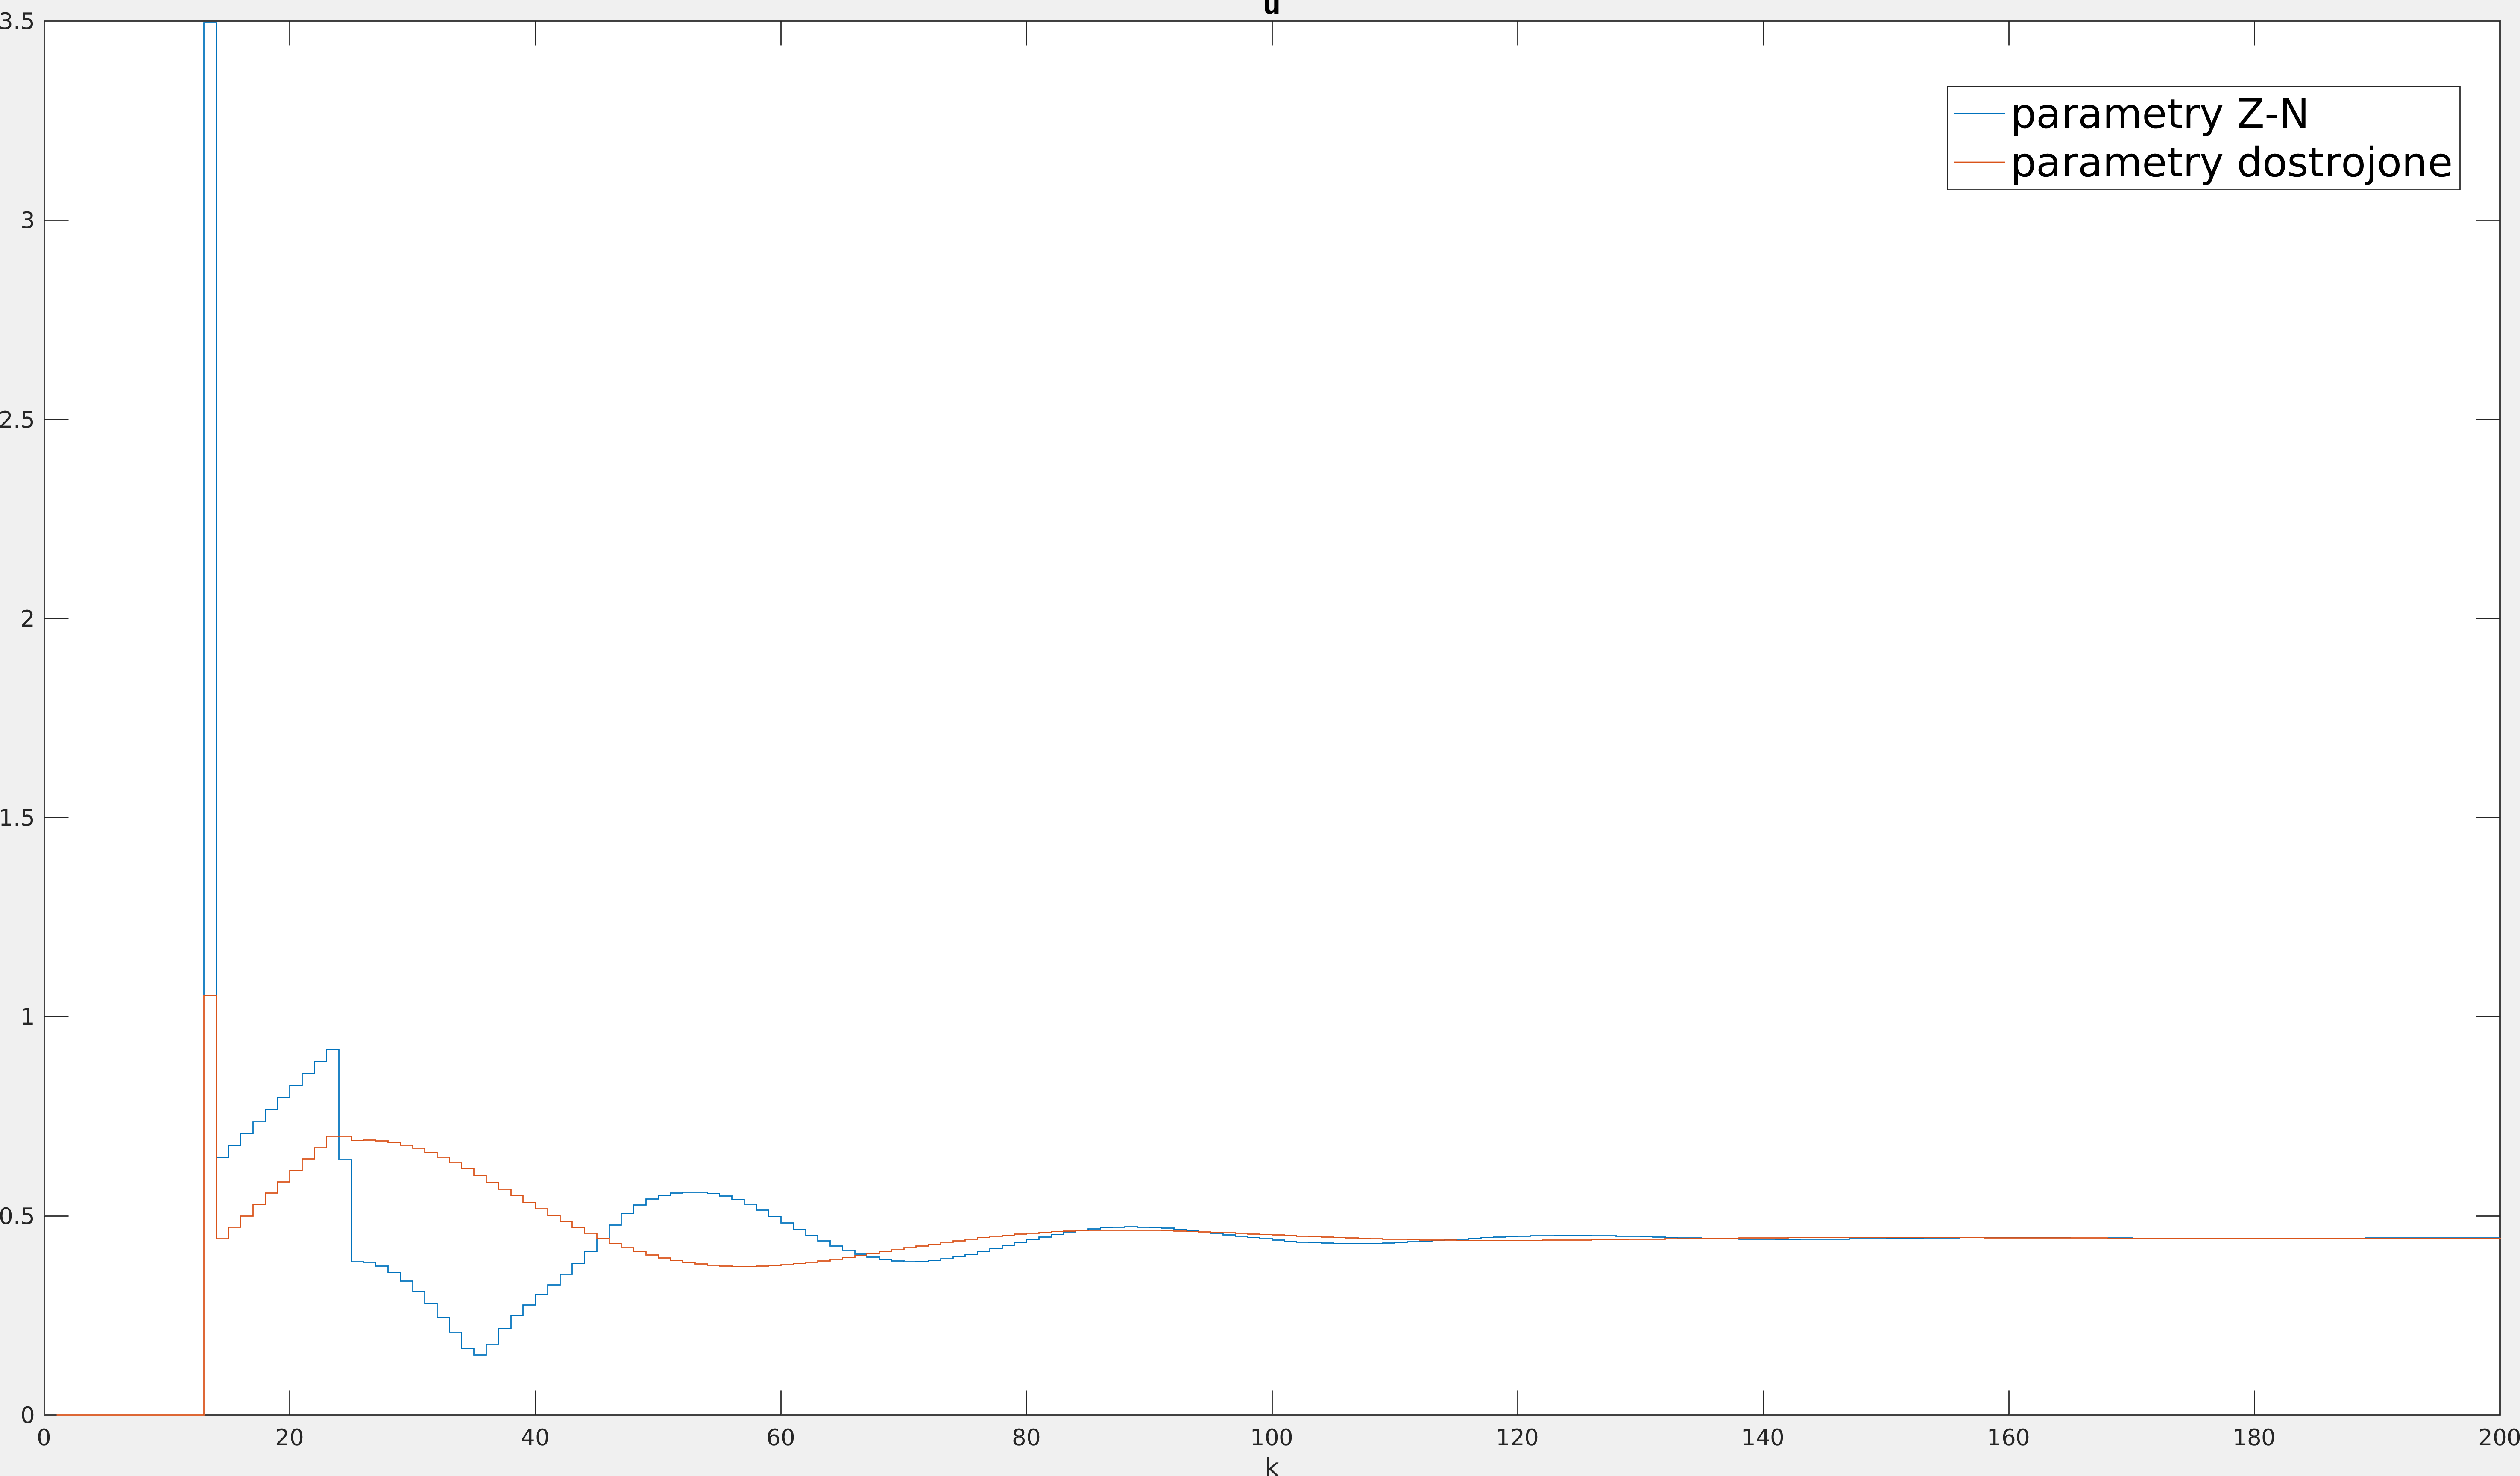
\includegraphics[width=\textwidth]{scripts/dyskretster.png}
	\caption{sygnał sterujący obiektu regulacji cyfrowej}
\end{figure}

Sygnał wyjściowy nie różni się zbytnio w przypadku początkowych nastaw i poprawionych, chociaż łagodniejsza odpowiedź i nieco krótszy czas regulacji przemawiają wciąż za wartościami dobranymi później. Dopiero wykres sygnału sterującego ukazuje zdecydowanie bardziej przyjazną trajektorię dla poprawionych współczynników, co ujawnia się trzykrotnie mniejszym skokiem sterowania na początku regulacji i łagodniejszym jego zmianom oraz szybszemu ustaleniu wartości.

\section{Regulator DMC}

Regulator DMC (Dynamic Matrix Control) jest jednym z przykładów algorytmów regulacji predykcyjnej. Stosowany jest do obiektów stabilnych, gdyż opiera się na wyznaczonej uprzednio odpowiedzi skokowej obiektu, a dokładniej na dyskretnych próbkach $S$ tej odpowiedzi. Ich zebranie to pierwszy punkt algorytmu. Zadaniem w projekcie było zaprojektowanie wersji analitycznej regulatora bez ograniczeń. Głównymi parametrami regulatora są parametry $D$, $N$ oraz $N_u$. Zostaną one omówione poniżej.

Przewidywana trajektoria obiektu regulacji wyraża się wyrażeniem wektorowym
{\Large
\begin{equation}
	\hat{Y}(k) = Y^o(k)+\Delta Y(k)
\end{equation}
}
gdzie $Y^o(k)$ nazywana jest odpowiedzią swobodną, a $Y(k)$ odpowiedzią wymuszoną.

\subsection{Odpowiedź swobodna}

Odpowiedź swobodną wyznacza się w sposób wektorowy korzystając z poniższego wzoru
{\Large
\begin{equation}
	 Y^o (k) = Y(k) + M^P \Delta U^P (k)
\end{equation}
}
gdzie $Y(k)$ to wektor $N$ aktualnych wyjść procesu, $M^P$ o wymiarowości $NxD-1$ to macierz postaci
{\Large
\begin{equation}
	M^P=\begin{bmatrix}
		s_2-s_1 & s_3-s_2 & \dots & s_D-s_{D-1}\\
		s_3-s_1 & s_4-s_2 & \dots & s_{D+1}-s_{D-1}\\
		\vdots & \vdots & \ddots & \vdots \\
		s_{N+1}-s_1 & s_{N+2}-s_2 & \dots	& s_{N+D-1}-s_{D-1}
	\end{bmatrix}
\end{equation}
}

natomiast wektor $\Delta U^p(k)$ to wektor przeszłych $D-1$ zmian sterowania.

\subsection{Odpowiedź wymuszona}

Drugą część równania $\hat{Y}(k)$ wyznacza się korzystając z Zależności
{\Large
\begin{equation}
	\Delta Y(k)=M\Delta U(k)
\end{equation}
}
gdzie $\Delta Y(k)$ to wektor różnicy wartości zadanej wyjścia obiektu i ostatniej wartości jego odpowiedzi, macierz $M$ o wymiarach $NxN_u$ wyznacza się ze wzoru

{\Large
\begin{equation}
	M=\begin{bmatrix}
		s_1 & 0 & \dots & 0 \\
		s_2 & s_1 & \dots & 0 \\
		\vdots & \vdots & \ddots & \vdots \\
		s_N & s_{N-1} & \dots & s_{N-N_u+1}
\end{bmatrix}
\end{equation}
}

natomiast wektor optymalnych zmian sterowań $\Delta U(k)$ wyznacza się korzystając ze wzoru

{\Large
\begin{equation}
	\Delta U(k)=(M^T\Psi M+\Lambda)^{-1}M^T\Psi (\Delta Y(k)-M^P\Delta U^P(k))
\end{equation}
}
Macierze diagonalne $\Psi$ oraz $\Lambda$ są głównymi parametrami dostrajania regulatora DMC. W przypadku zadania projektowego ustalono macierz $\Psi$ jako macierz jednostkową $I$, macierz $\Lambda$ będzie później wykorzystana przy ograniczaniu zmian sterowania.

\section{Dobieranie regulatora DMC}

Dobieranie regulatora polega na wyznaczeniu wartości parametrów
\begin{itemize}
	\item $D$ - horyzont dynamiki - ilość próbek, po których odpowiedź skokowa obiektu ustala się na jednej wartości
	\item $N$ - horyzont predykcji
	\item $N_u$ - horyzont sterowania
\end{itemize}

Pierwszym krokiem, jak już zostało zaznaczone, jest wyznaczenie dyskretnych wartości odpowiedzi skokowej obiektu, a następnie na jej podstawie wyznaczenie horyzontu dynamiki.

W przypadku obiektu o parametrach z zadania $2.29$ odpowiedź skokowa ma następującą postać

\begin{figure}[H]
	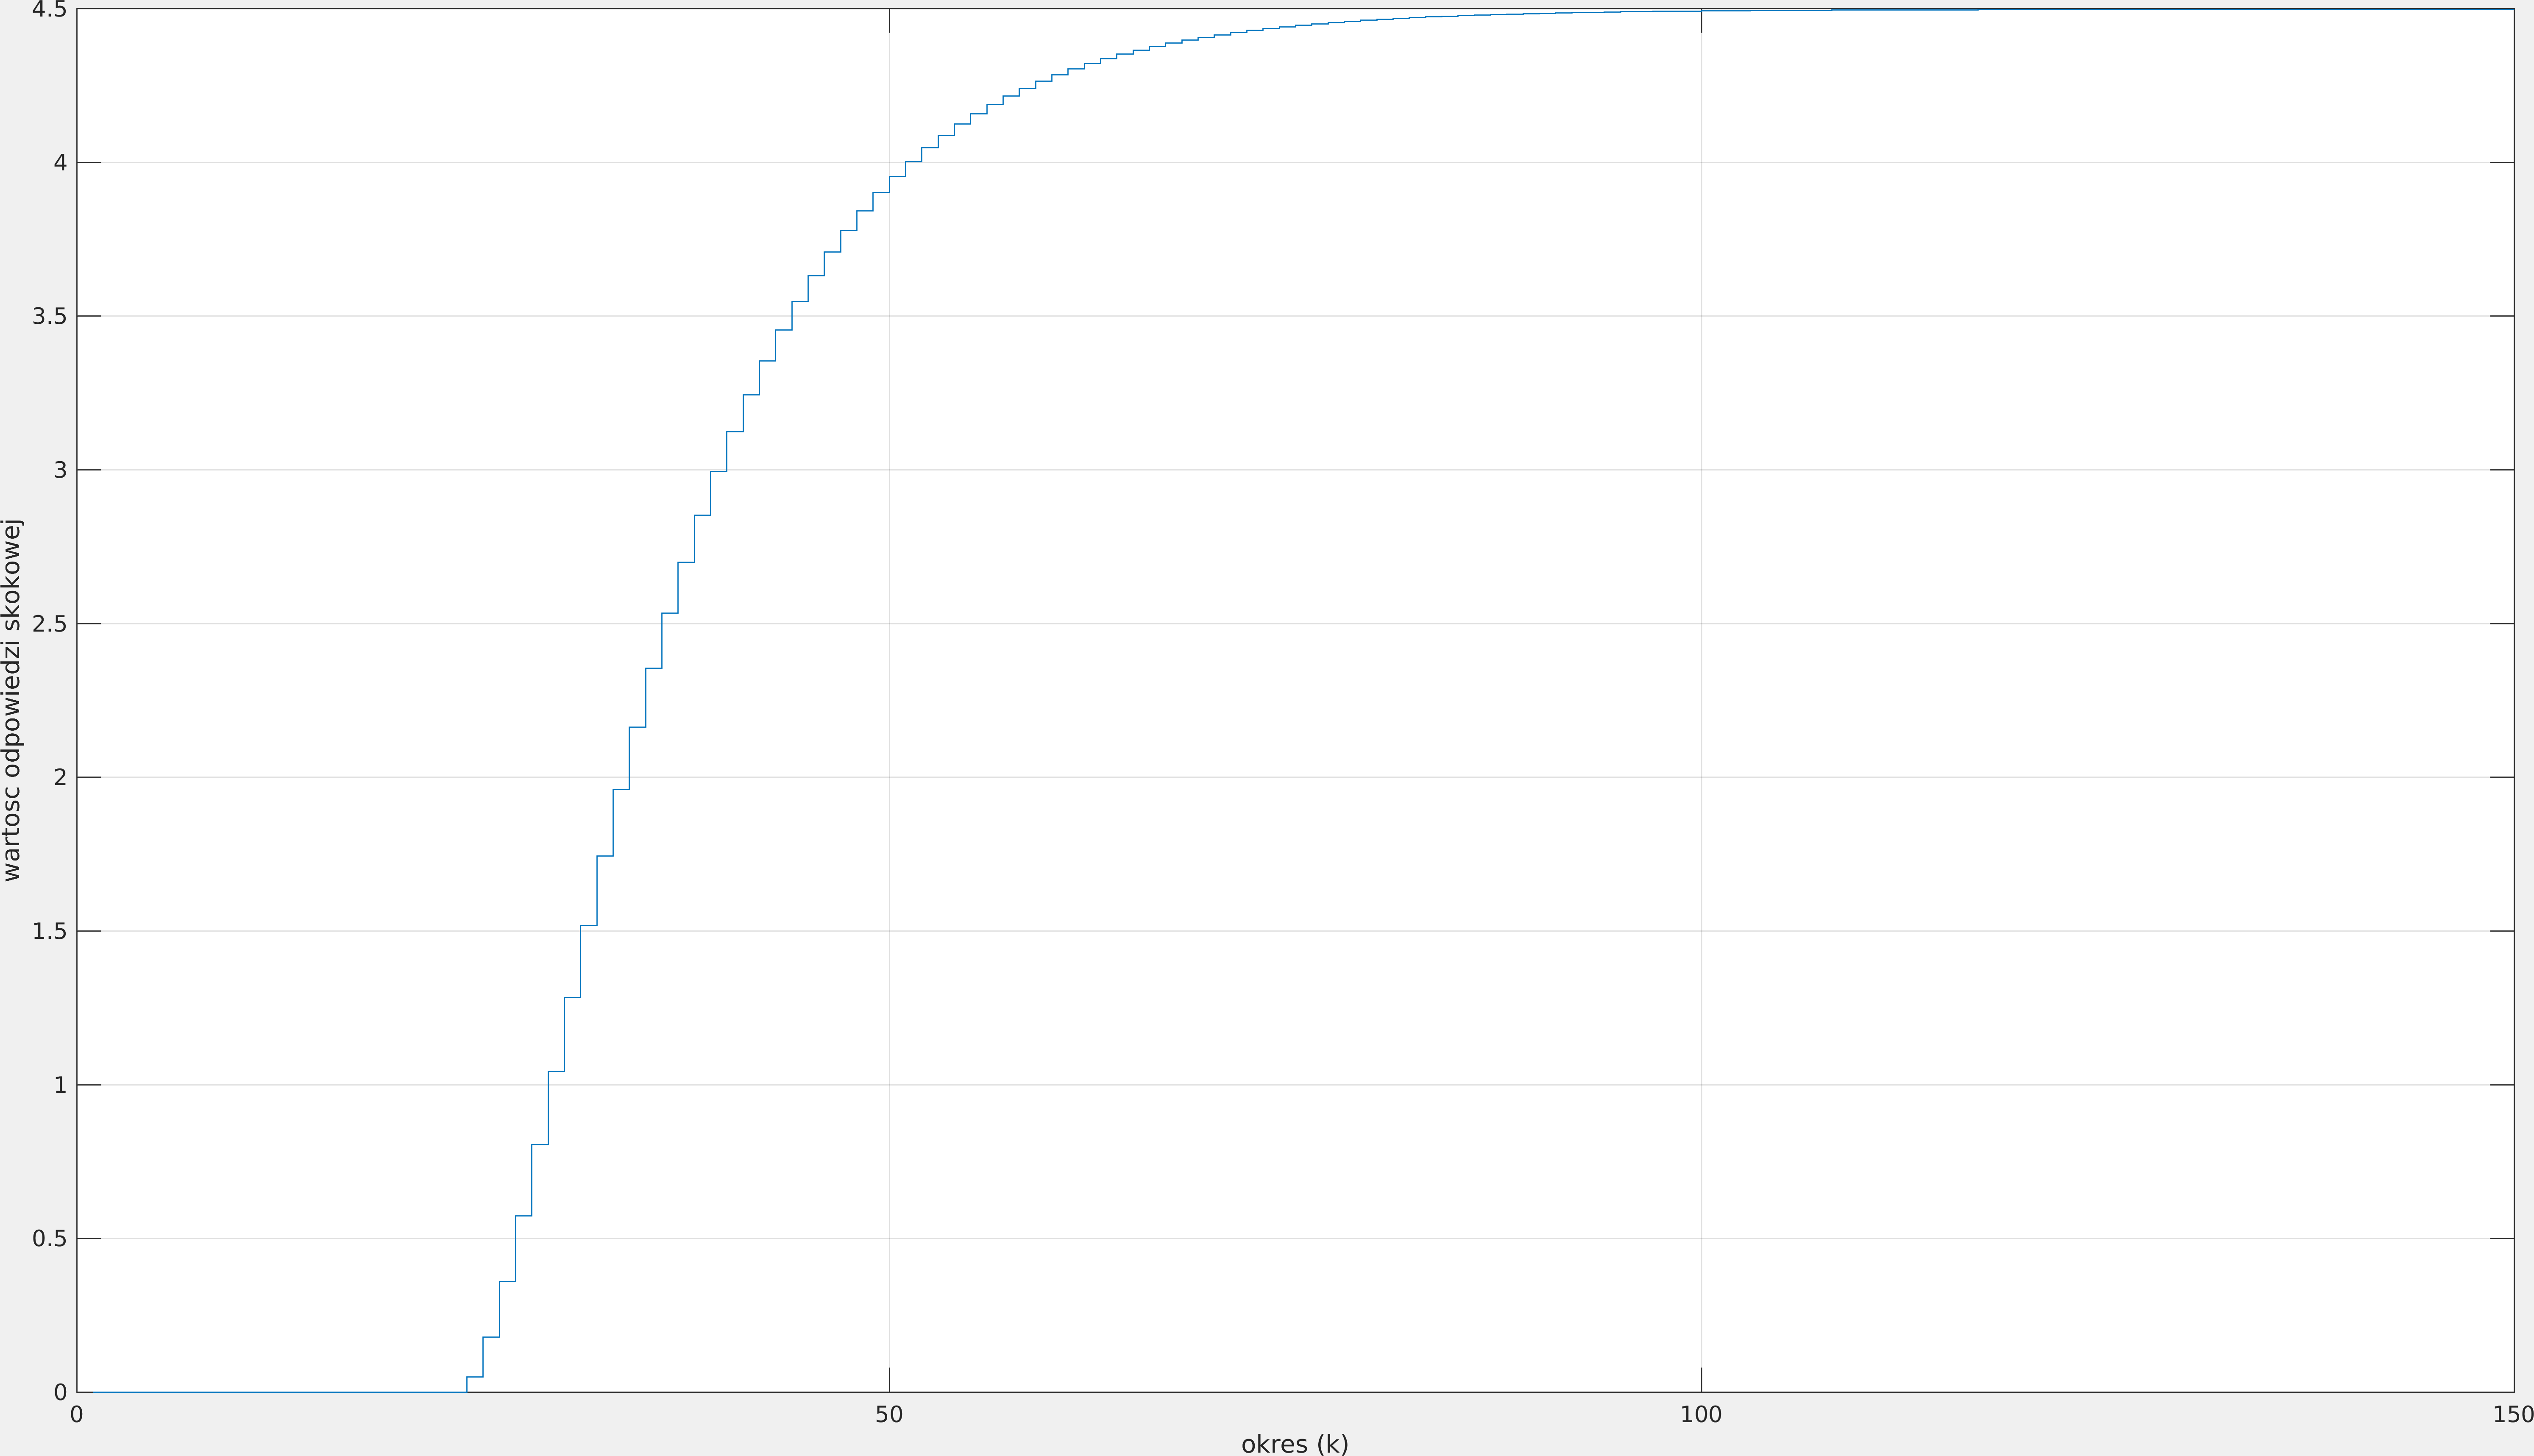
\includegraphics[width=\textwidth]{scripts/odpskokdys.png}
	\caption{dyskretna odpowiedź skokowa obiektu}
\end{figure}

\subsection{Wyznaczanie horyzontu dynamiki}


Po przeanalizowaniu powyższego wykresu ustalono wartość horyzontu dynamiki na $125$. Ustawiono wartości parametrów $N$ i $N_u$ na tą samą wartość, wartość współczynnika $\lambda$ macierzy $\Lambda$ ustalono początkowo na wartość $1$ i przetestowano jakość algorytmu. Wyniki eksperymentu znajdują się Poniżej

\begin{figure}[H]
	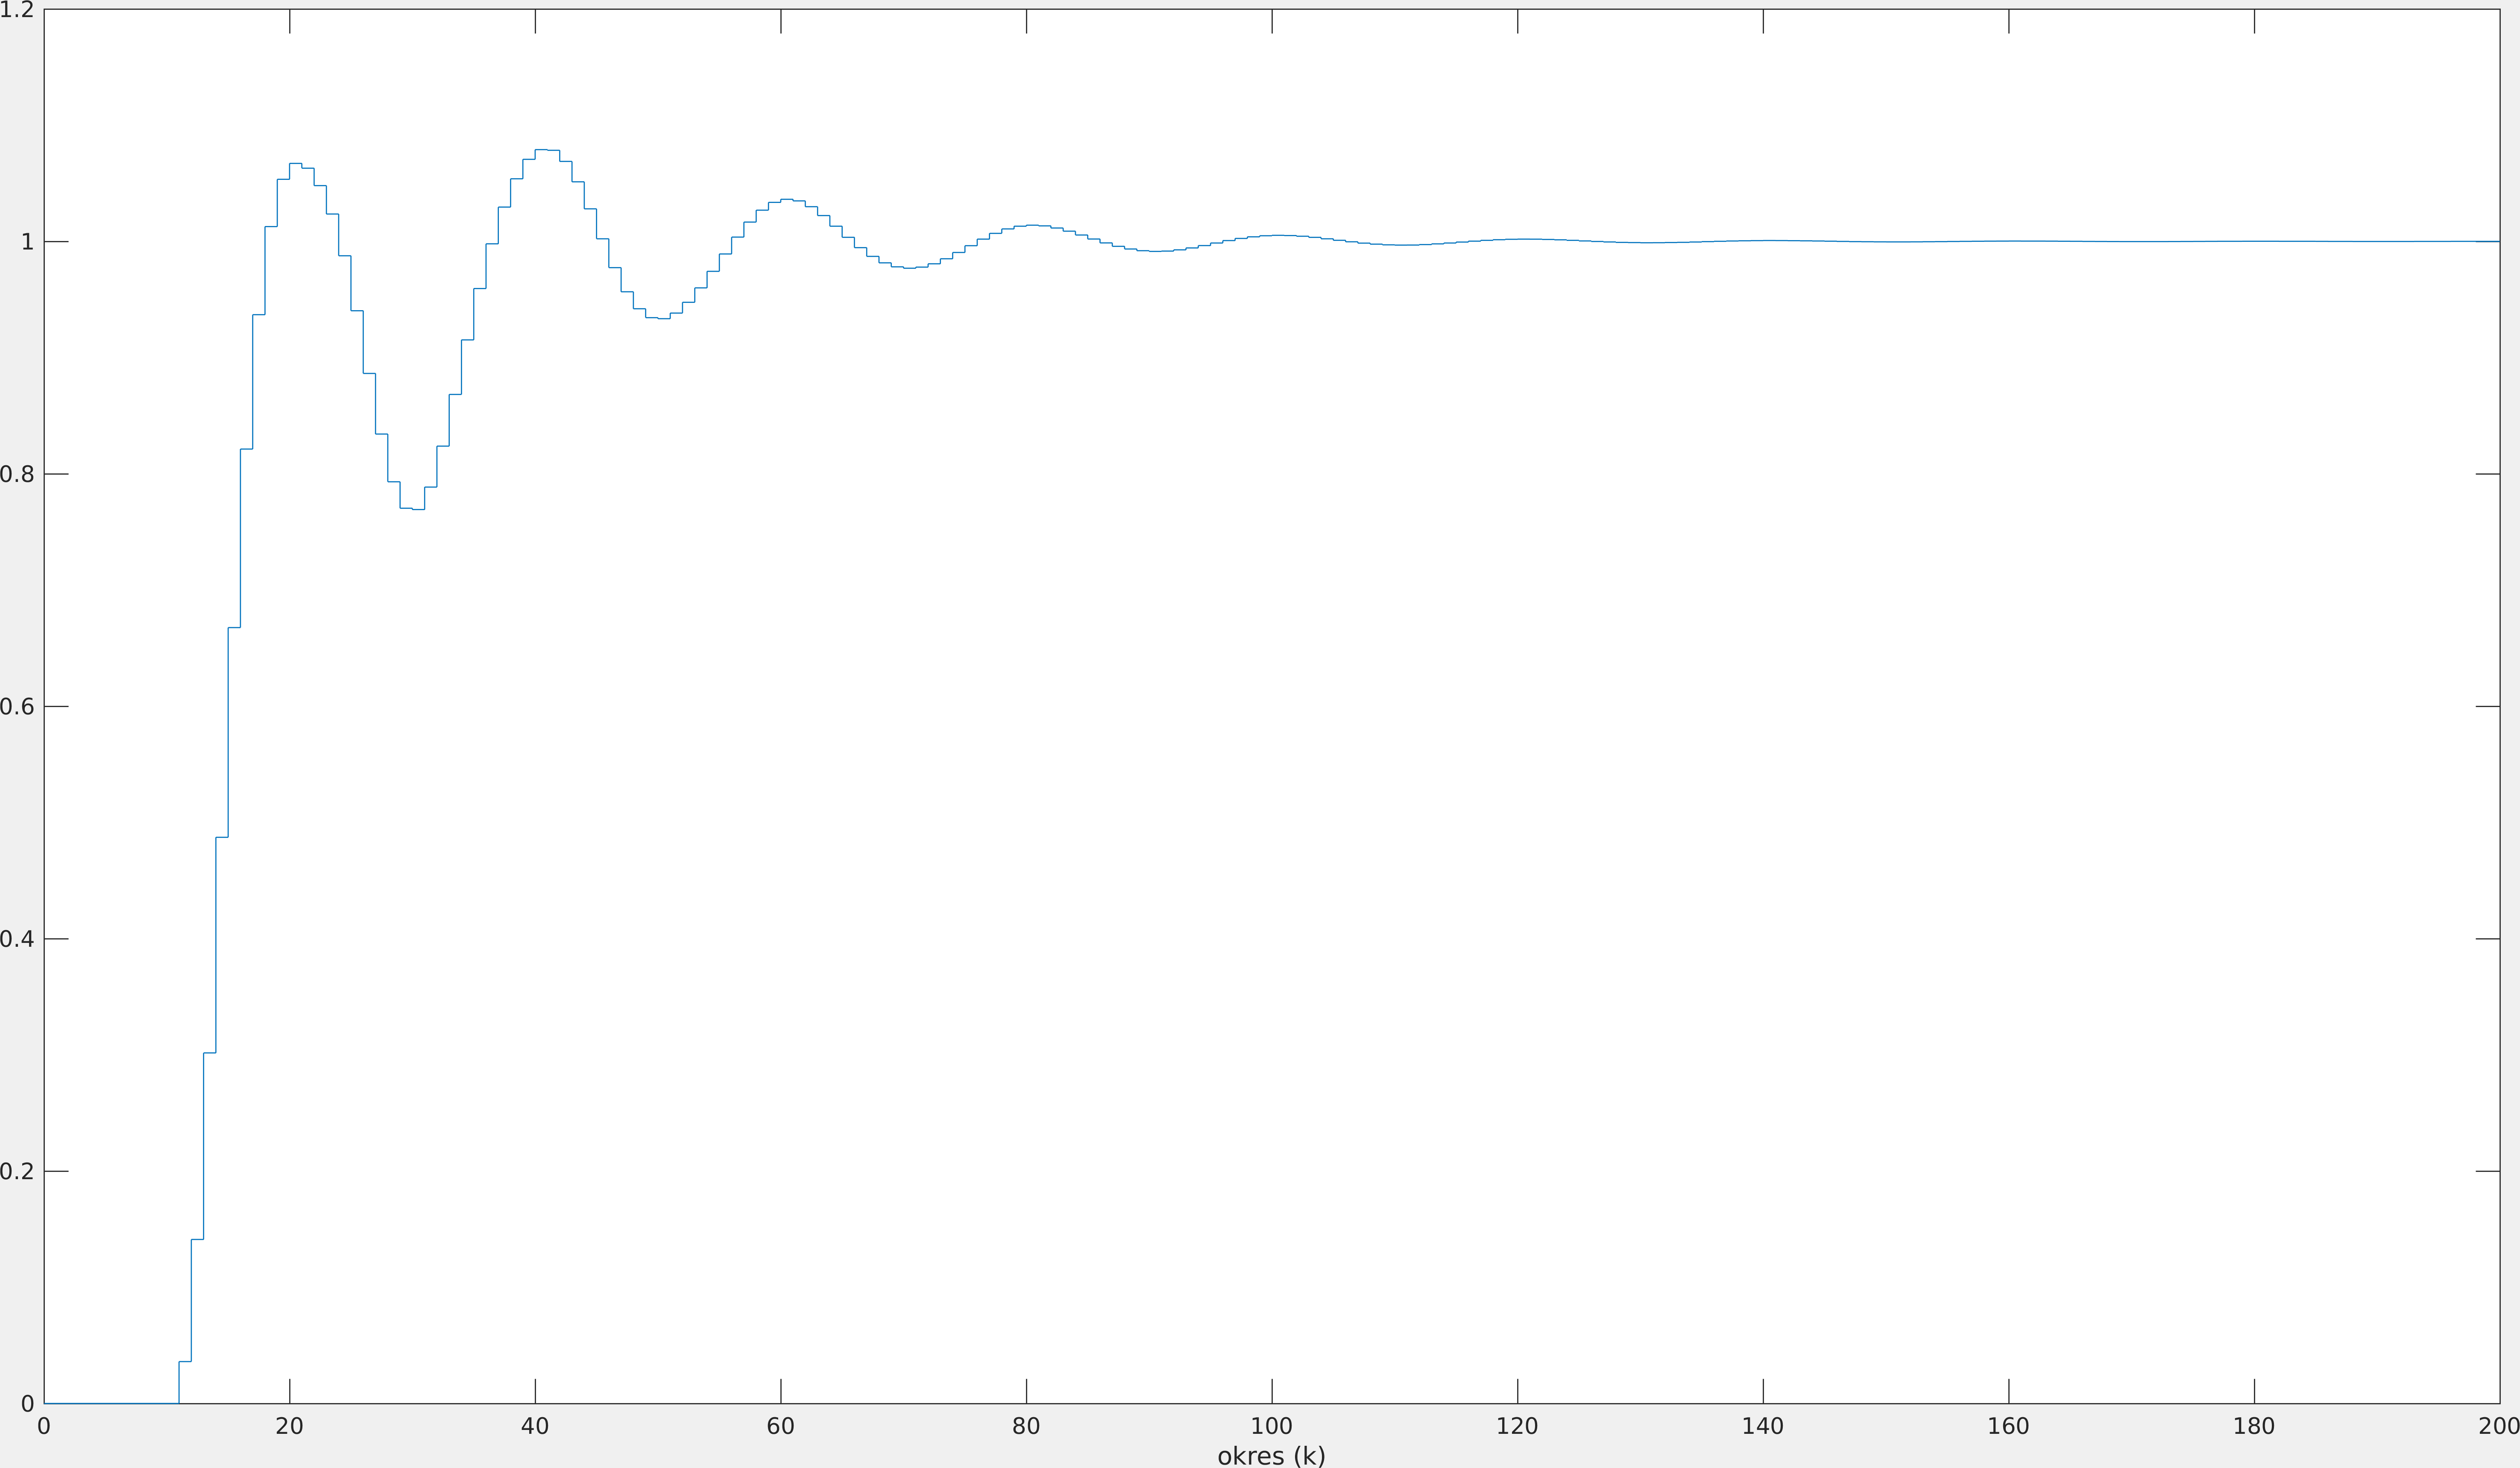
\includegraphics[width=\textwidth]{scripts/regDDD2.png}
	\caption{odpowiedź obiektu regulacji przy nastawach $125, 125, 125, 1$}
\end{figure}
\begin{figure}[H]
	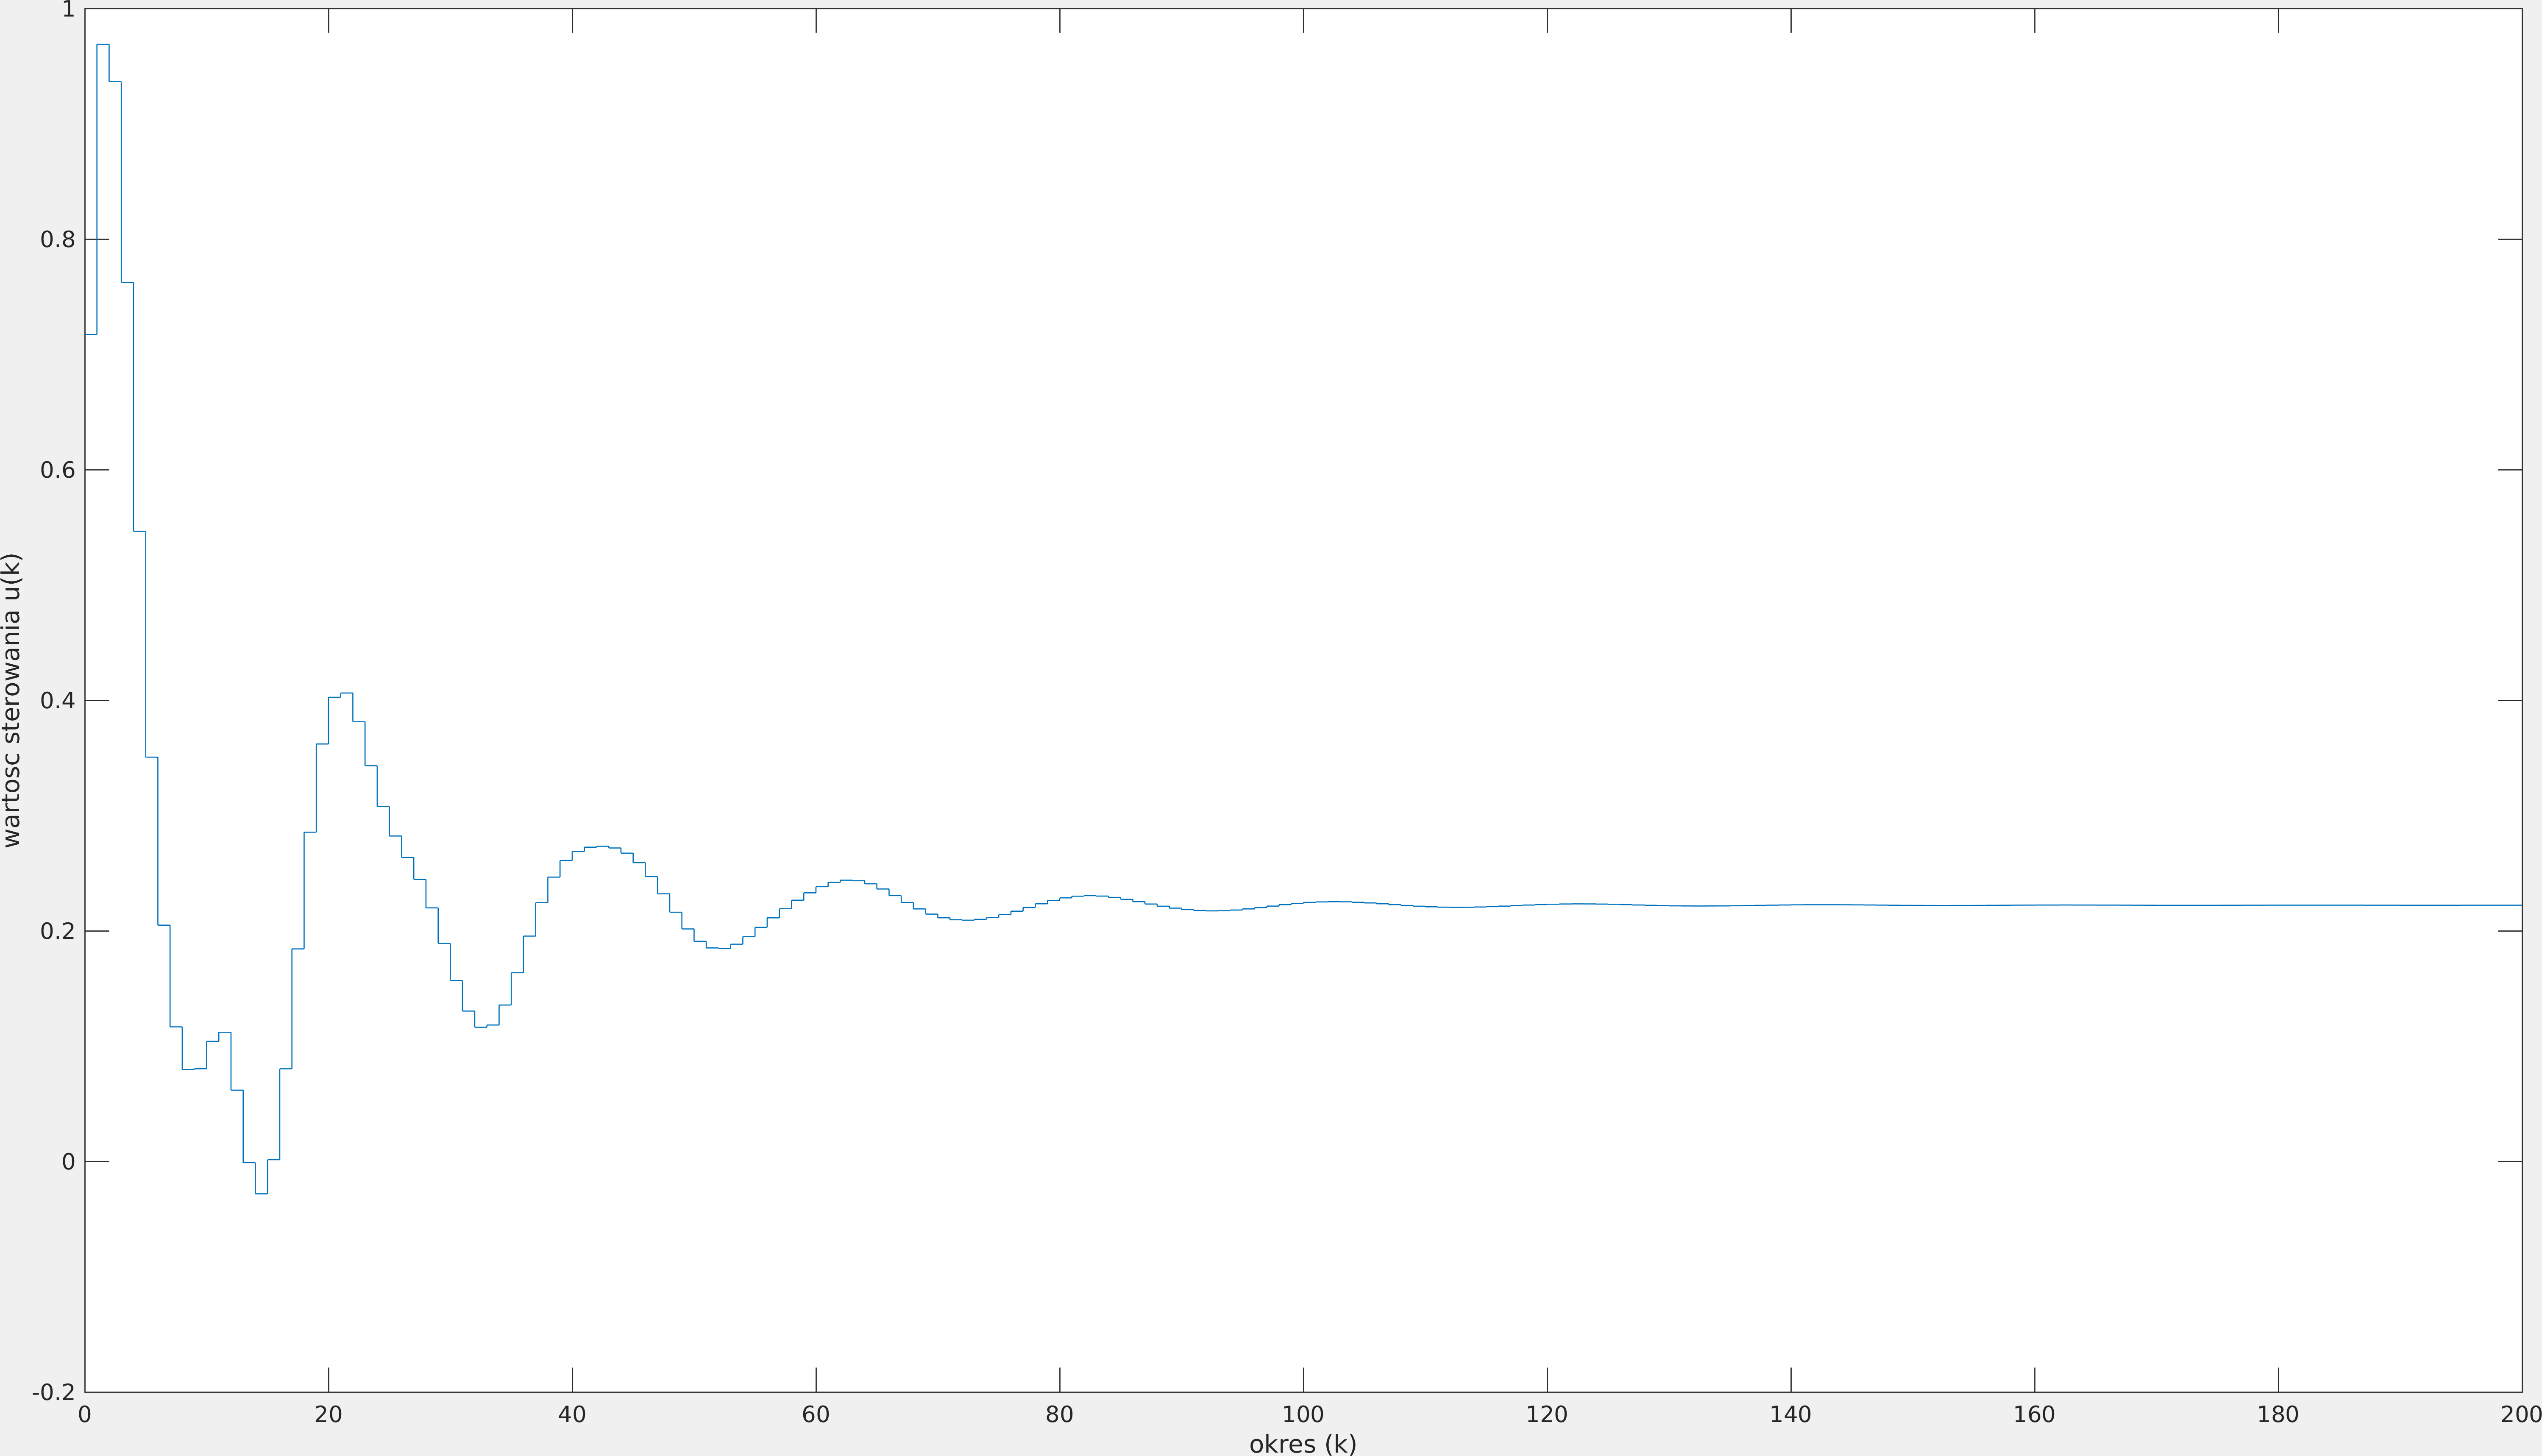
\includegraphics[width=\textwidth]{scripts/regDDDster2.png}
	\caption{sygnał sterujący przy nastawach $125, 125, 125, 1$}
	\label{}
\end{figure}

Jak widać regulator został poprawnie zaprojektowany, podstawowe nastawy parametrów powodują stosunkowo szybką regulację z szybko gasnącymi oscylacjami. Dalszą częscią zadania było ograniczenie wartości parametru horyzontu predykcji, co znacząco zmniejszyło nakład obliczeń algorytmu dzięki mniejszym wektorom i macierzom.

\subsection{Wyznaczanie horyzontu predykcji}

%TODO poprawić wybraną wartość
Przeprowadzono kilka testów i ostatecznie zdecydowano na wybranie wartości z okolic $20$. Powyżej niej nie miała miejsca żadna zmiana sygnału sterującego bądź wyjścia obiektu. Poniżej przedstawiono kilka odpowiedzi dla różnych wartości z okolic tej liczby. Wartość horyzontu dynamiki pozostała niemzieniona, tak samo wartość parametru $\lambda$. Przyjęto też $N_u=N$.

\begin{figure}[H]
	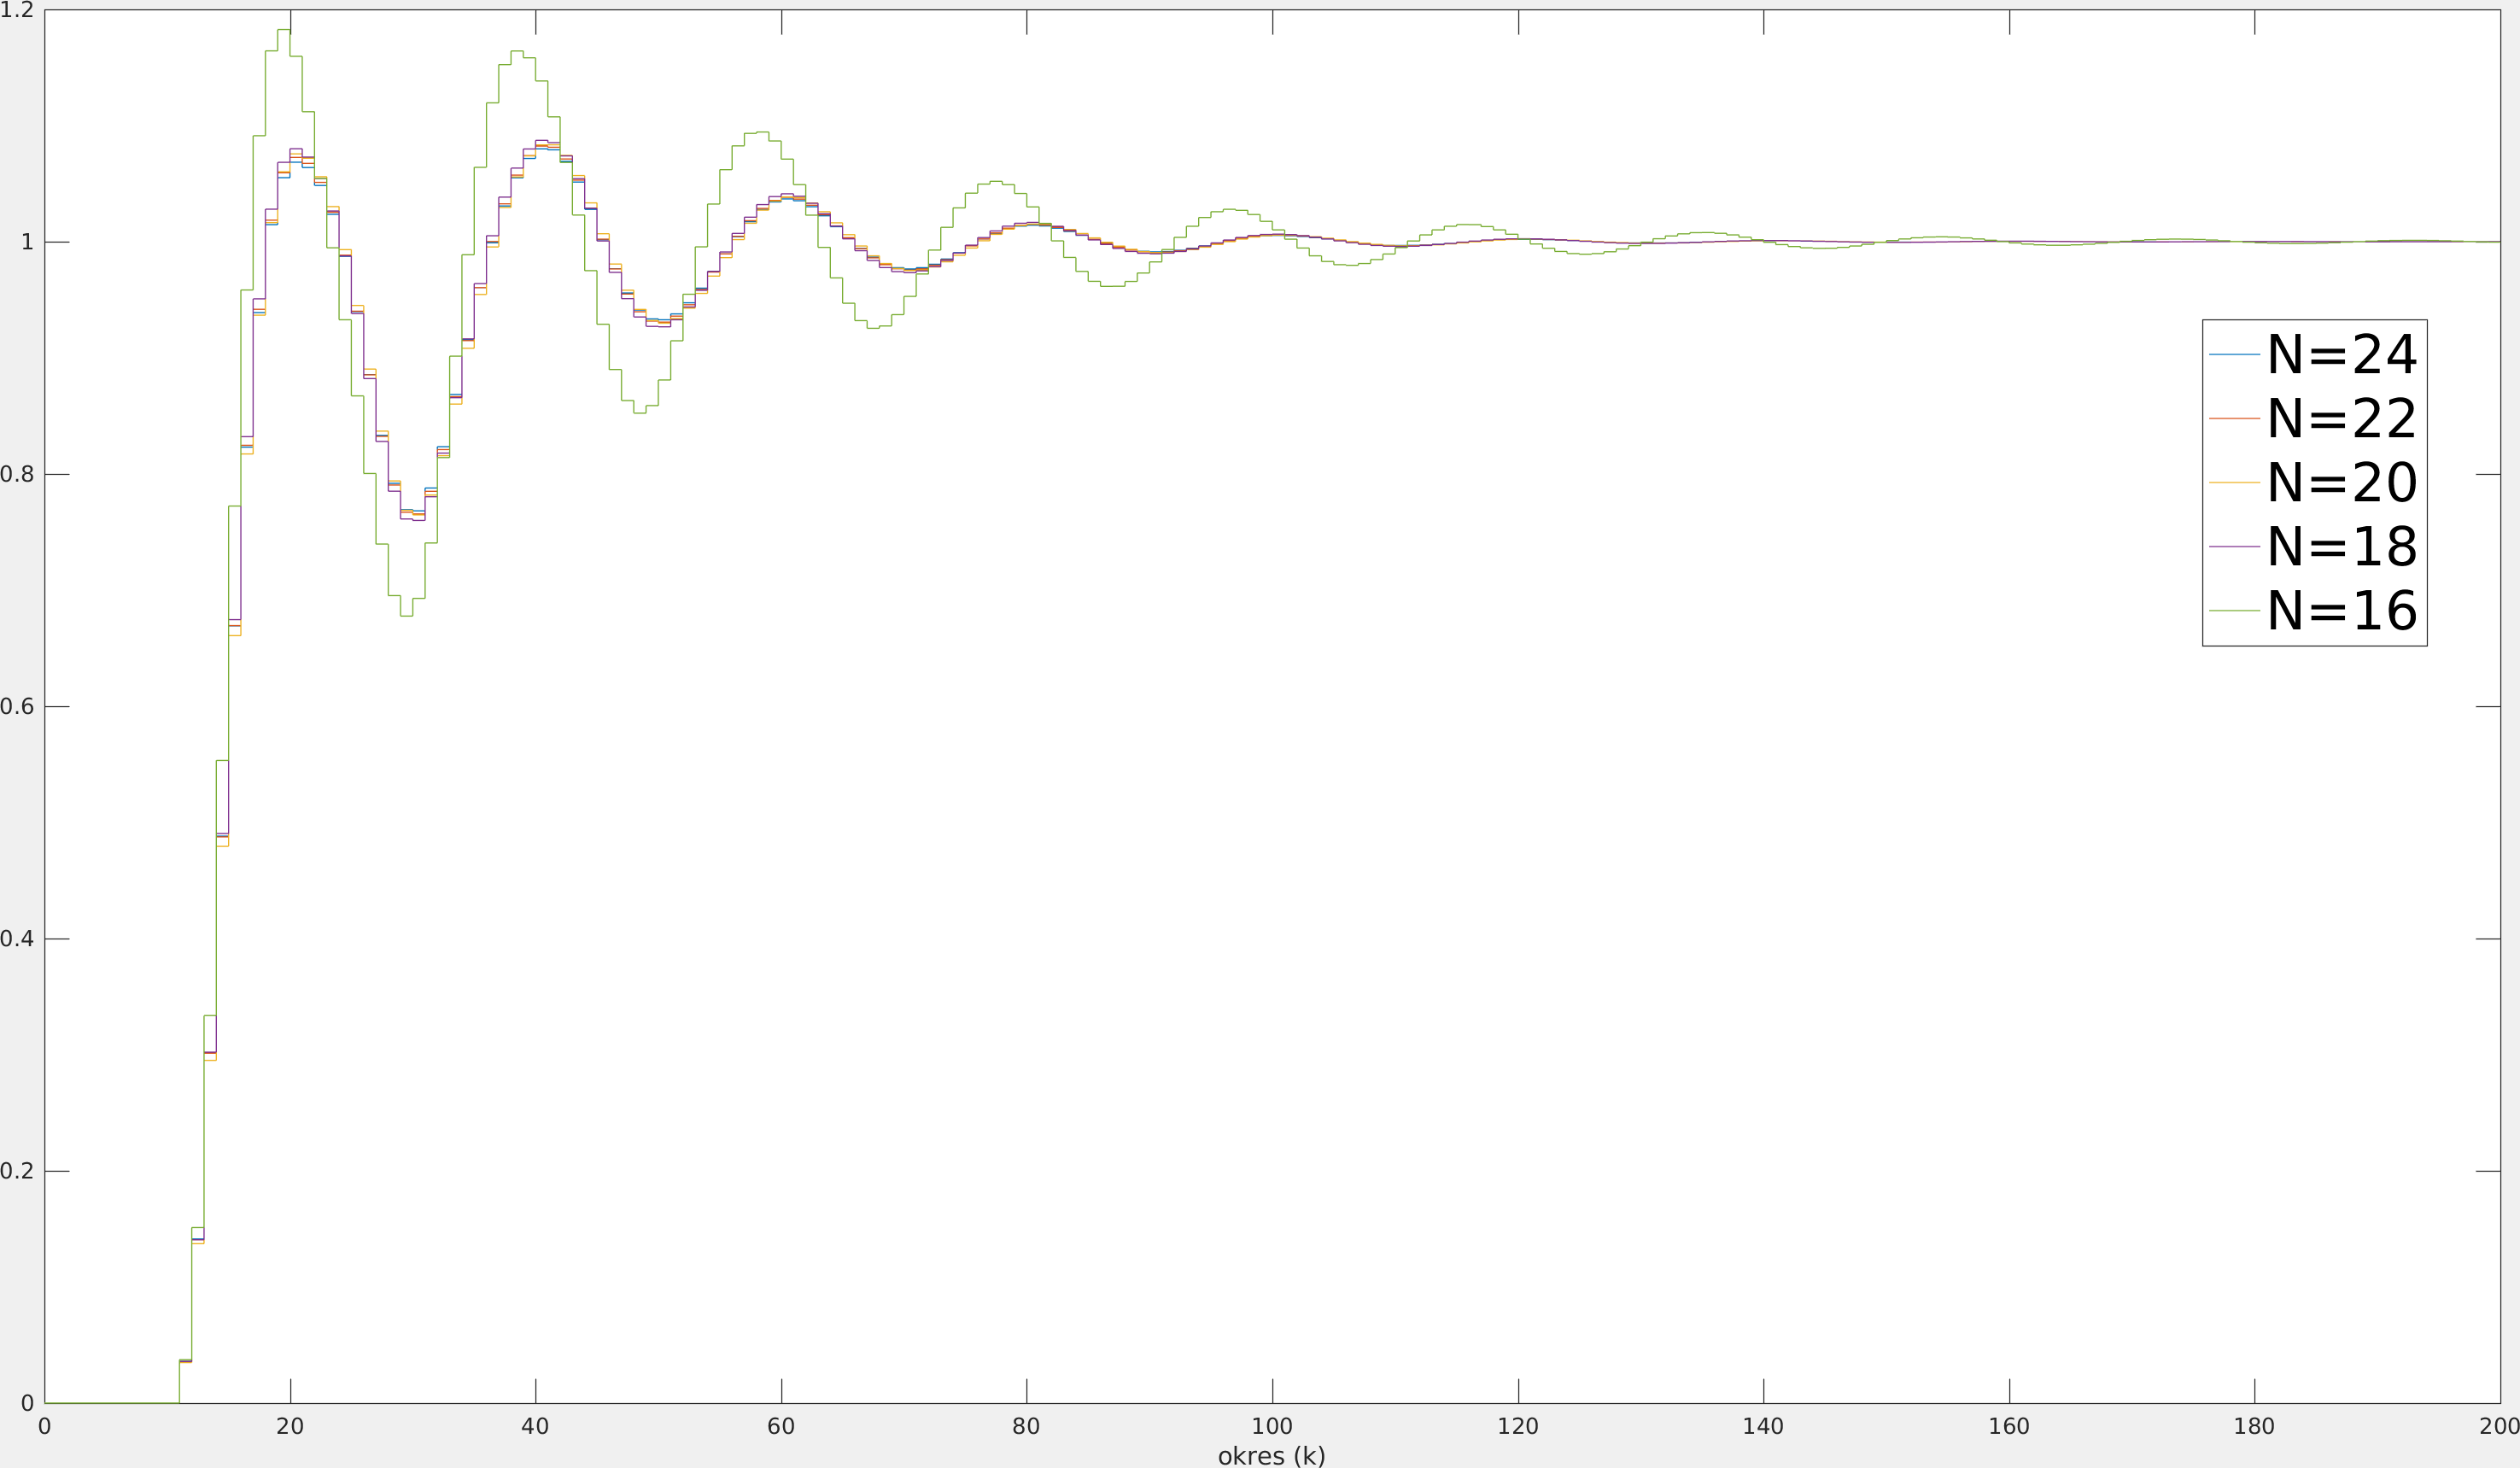
\includegraphics[width=\textwidth]{scripts/zadanie5bwyjscie2.png}
	\caption{odpowiedź obiektu regulacji dla parametrów $N$ oraz $N_u$ w okolicach 20}
\end{figure}
\begin{figure}[H]
	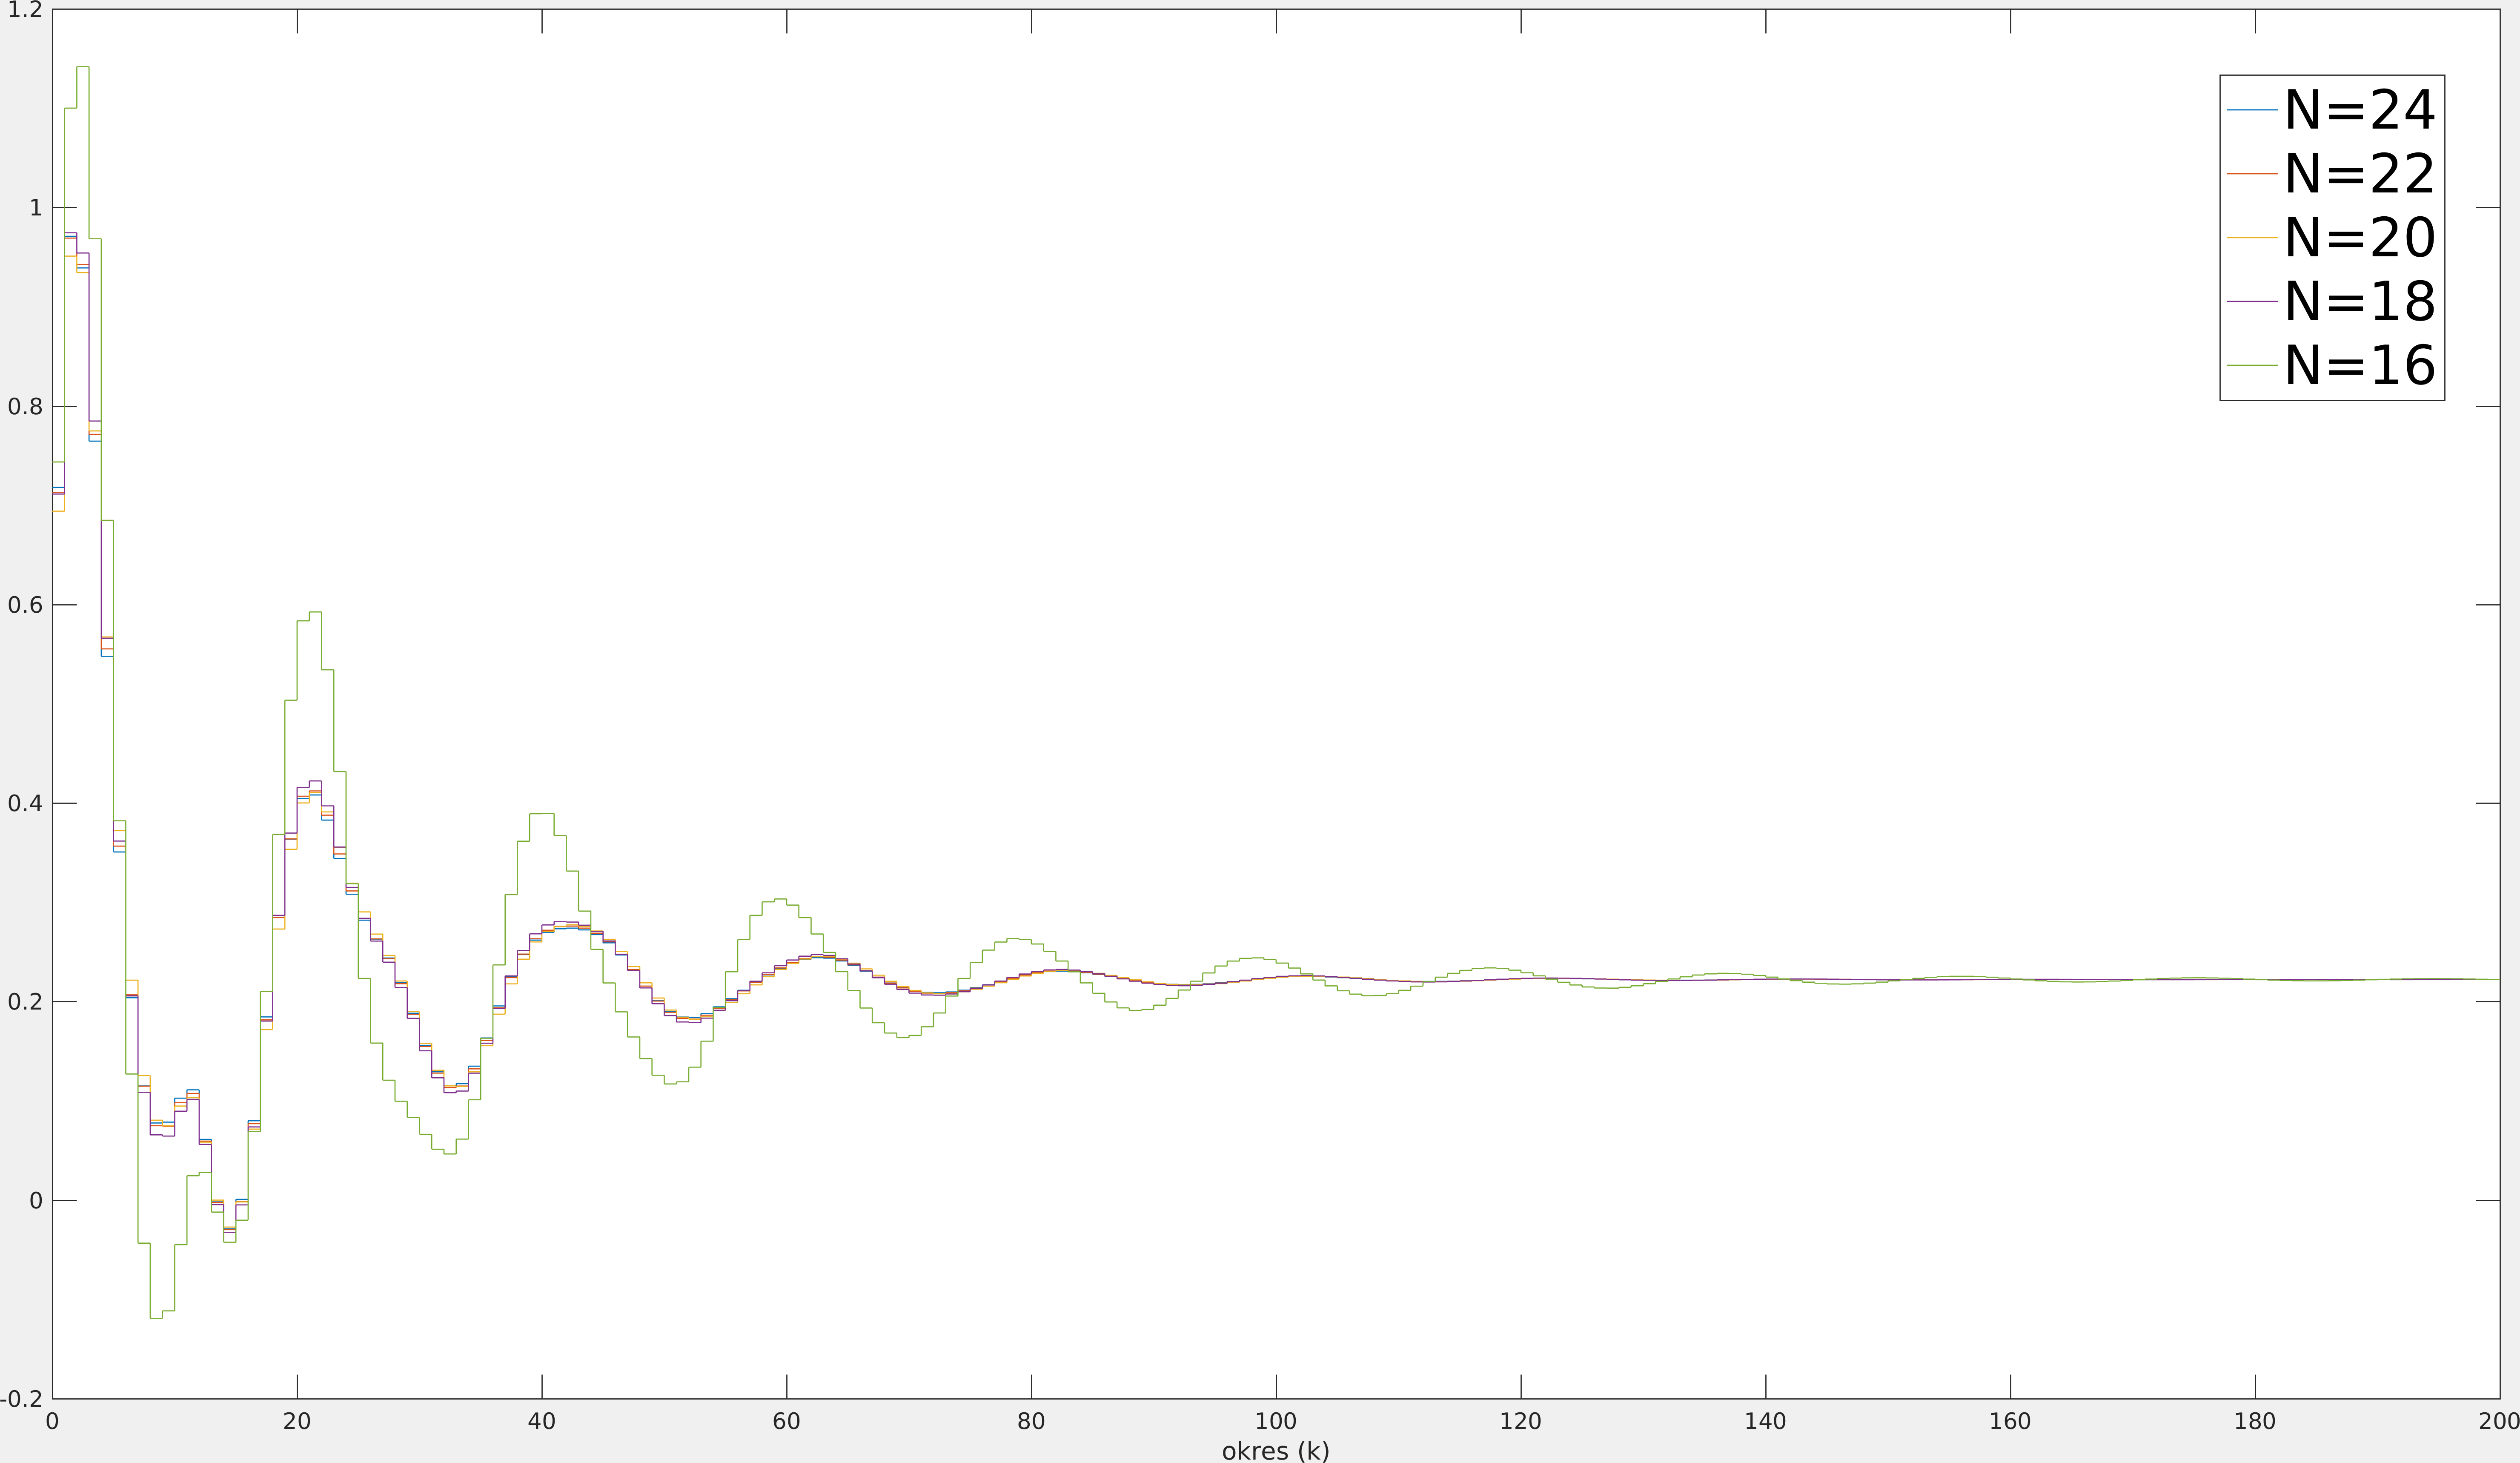
\includegraphics[width=\textwidth]{scripts/zadanie5bster2.png}
	\caption{sygnał sterujący obiektu regulacji dla parametrów $N$ oraz $N_u$ w okolicach 20}
\end{figure}

Jak widać wartości w granicach $(24;18)$ są bardzo zbliżone, jednak zdecydowano się pozostawić wartość horyzontu predykcji na $20$, gdyż powoduje w miarę niewielkie zmiany sterowania i dosyć szybką regulację obiektu sterowania. Wyraźnie widać, że wybranie horyzontu mniejszego niż $18$ powodowało by zdecydowanie większe oscylacje i dłuższy czas regulacji niż większe wartości- po przekroczeniu tej granicy regulator traci powoli zdolności regulacji, posiada za mało danych, aby operować w sposób optymalny. Z kolei większe wartości wciąż oscylowały w okolicach tej samej odpowiedzi, co widać dzięki podobieństwu nastaw początkowych $(125, 125, 125, 1)$, które uzyskały podobną odpowiedź co nastawy ostatecznie wybrane. Widać więc, że regulator nie wymaga więcej danych, aby operować zgodnie z oczekiwaniami.

\subsection{Wyznaczanie horyzontu sterowania}


Następnym punktem doboru nastaw było wybranie odpowiedniej wartości horyzontu sterowania. Przy wartościach pozostałych parametrów ustalonych w poprzednim punkcie rozpoczęto badania współczynnika od $1$ i kilku następnych wartości.

\begin{figure}[H]
	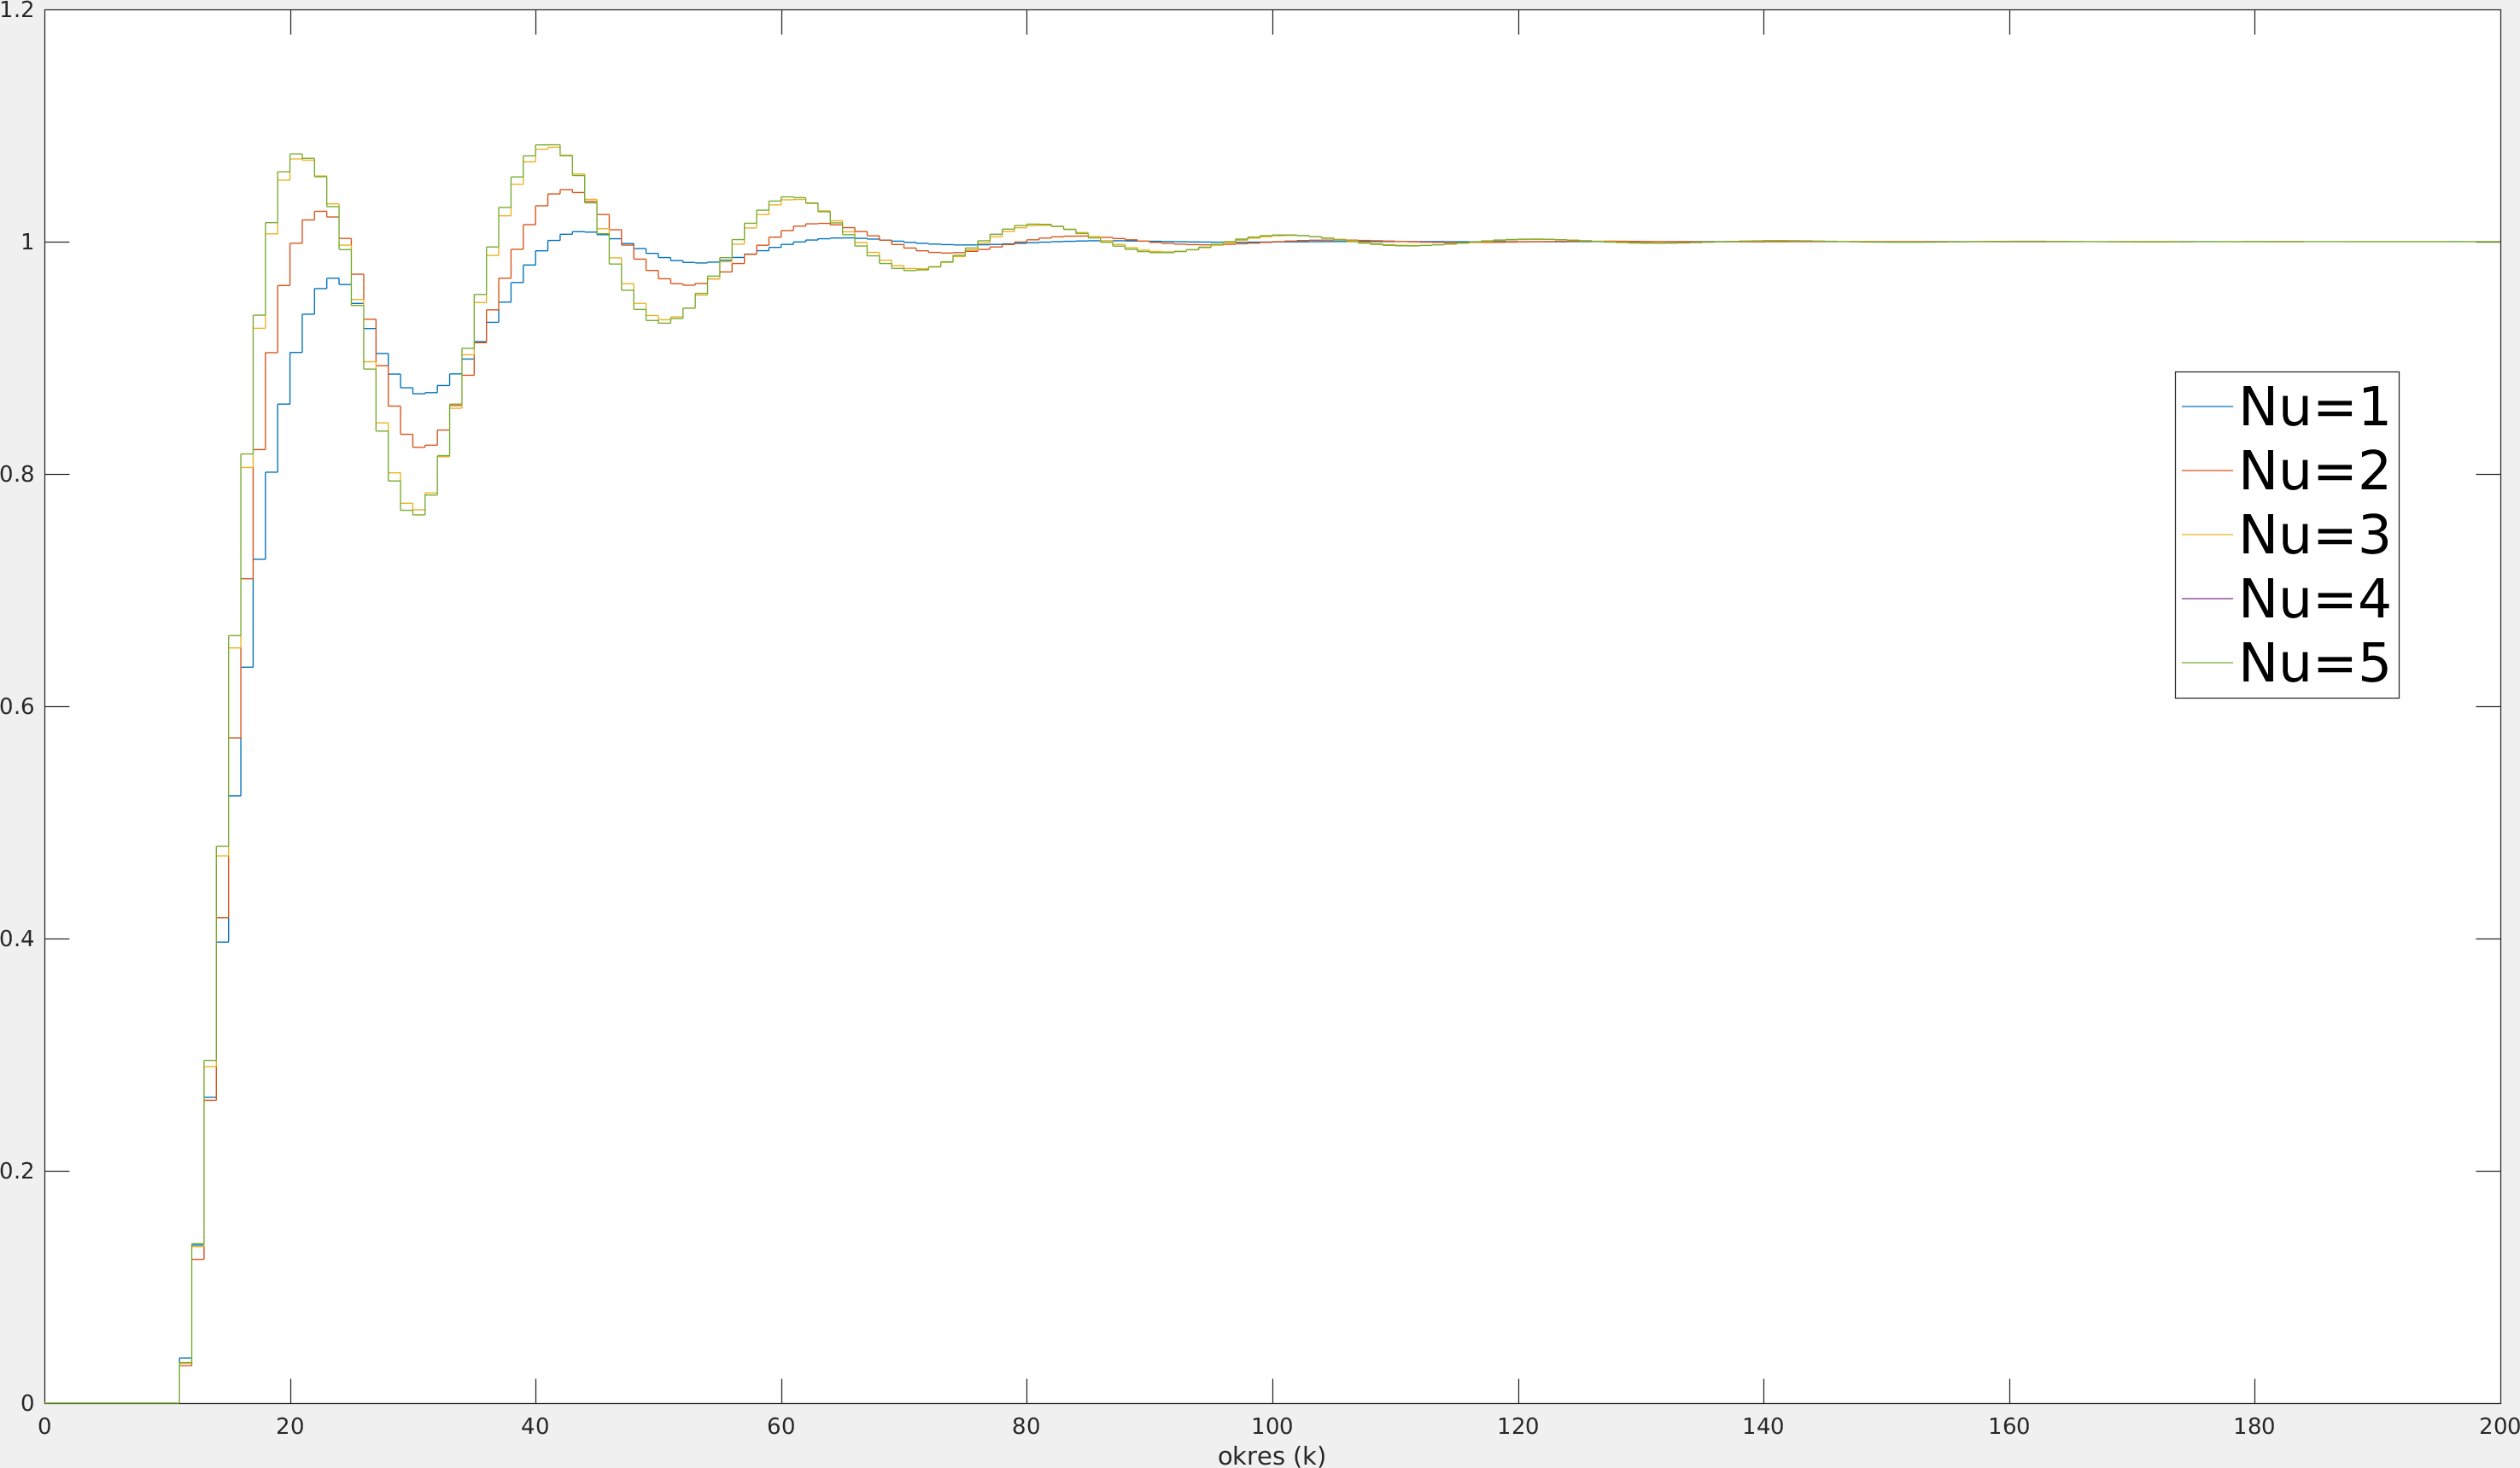
\includegraphics[width=\textwidth]{scripts/zadanie5cwyjscie2.png}
	\caption{odpowiedź obiektu regulacji dla różnych długości horyzontu sterowania}
\end{figure}
\begin{figure}[H]
	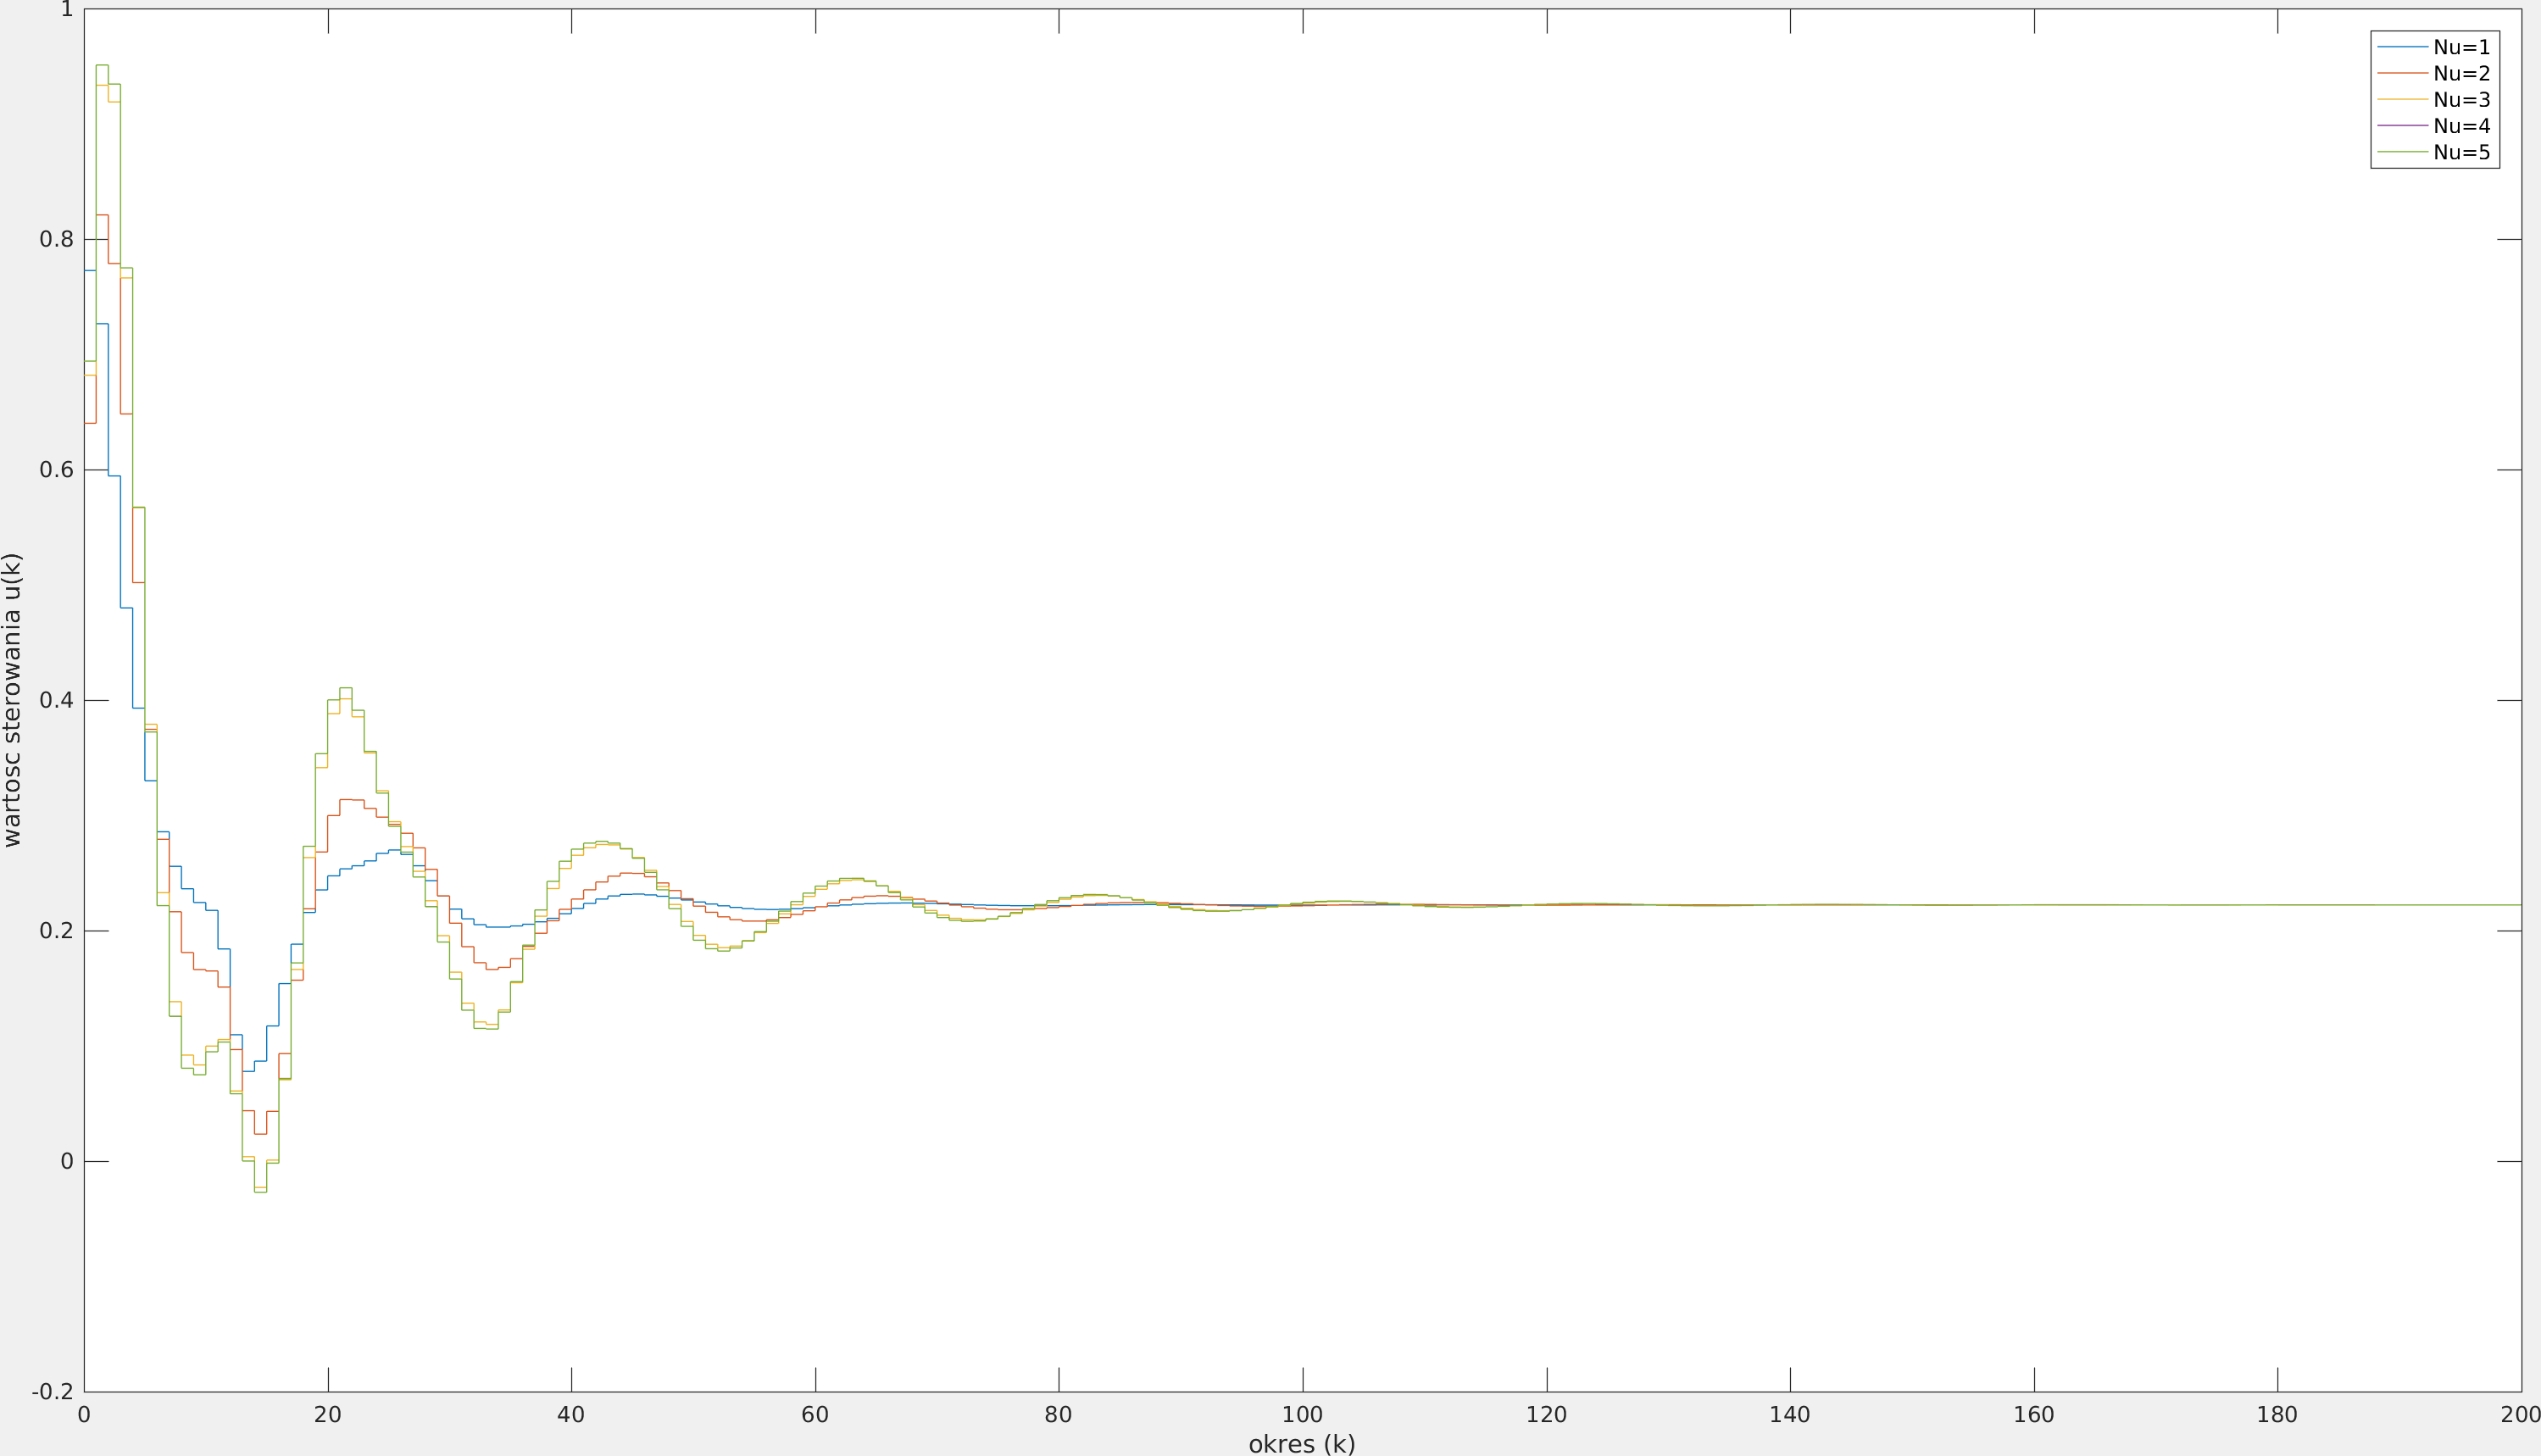
\includegraphics[width=\textwidth]{scripts/zadanie5cster2.png}
	\caption{wyjście sterowania obiektu regulacji dla różnych długości horyzontu sterowania}
\end{figure}

Na podstawie powyższych wykresów można wysnuć interesujący wniosek. Najlepsza jakość regulacji odpowiada horyzontowi sterowania równemu $1$. Zarówno odpowiedź obiektu, jak i wartość sterowania najszybciej się stabilizują i nie mają przeregulowania. Jedynym problemem może być duża wartość początkowa sygnału sterującego, lecz i tak jest ona zdecydowanie mniejsza niż w przypadku horyzontu sterowania o długości $20$. Można wysnuć wniosek, że próba wyskoczenia zbyt daleko do przodu w tym przypadku szkodzi optylmalnej regulacji obiektu. Pozwala to jednak dodatkowo zminimalizować nakład obliczeń z pozytywnym wpływem na jakość regulacji.

\subsection{Badanie parametru $\lambda$}

	Parametr $\lambda$ ma za zadanie ograniczyć wartość sygnału sterującego. ponieważ  Zmiany jednostkowe nie przynosiły prawie żadnych zmian, zdecydowano się na wybranie kilku wartości z przedziału $[5;45]$. Wyniki znajdują się poniżej.

	\begin{figure}[H]
		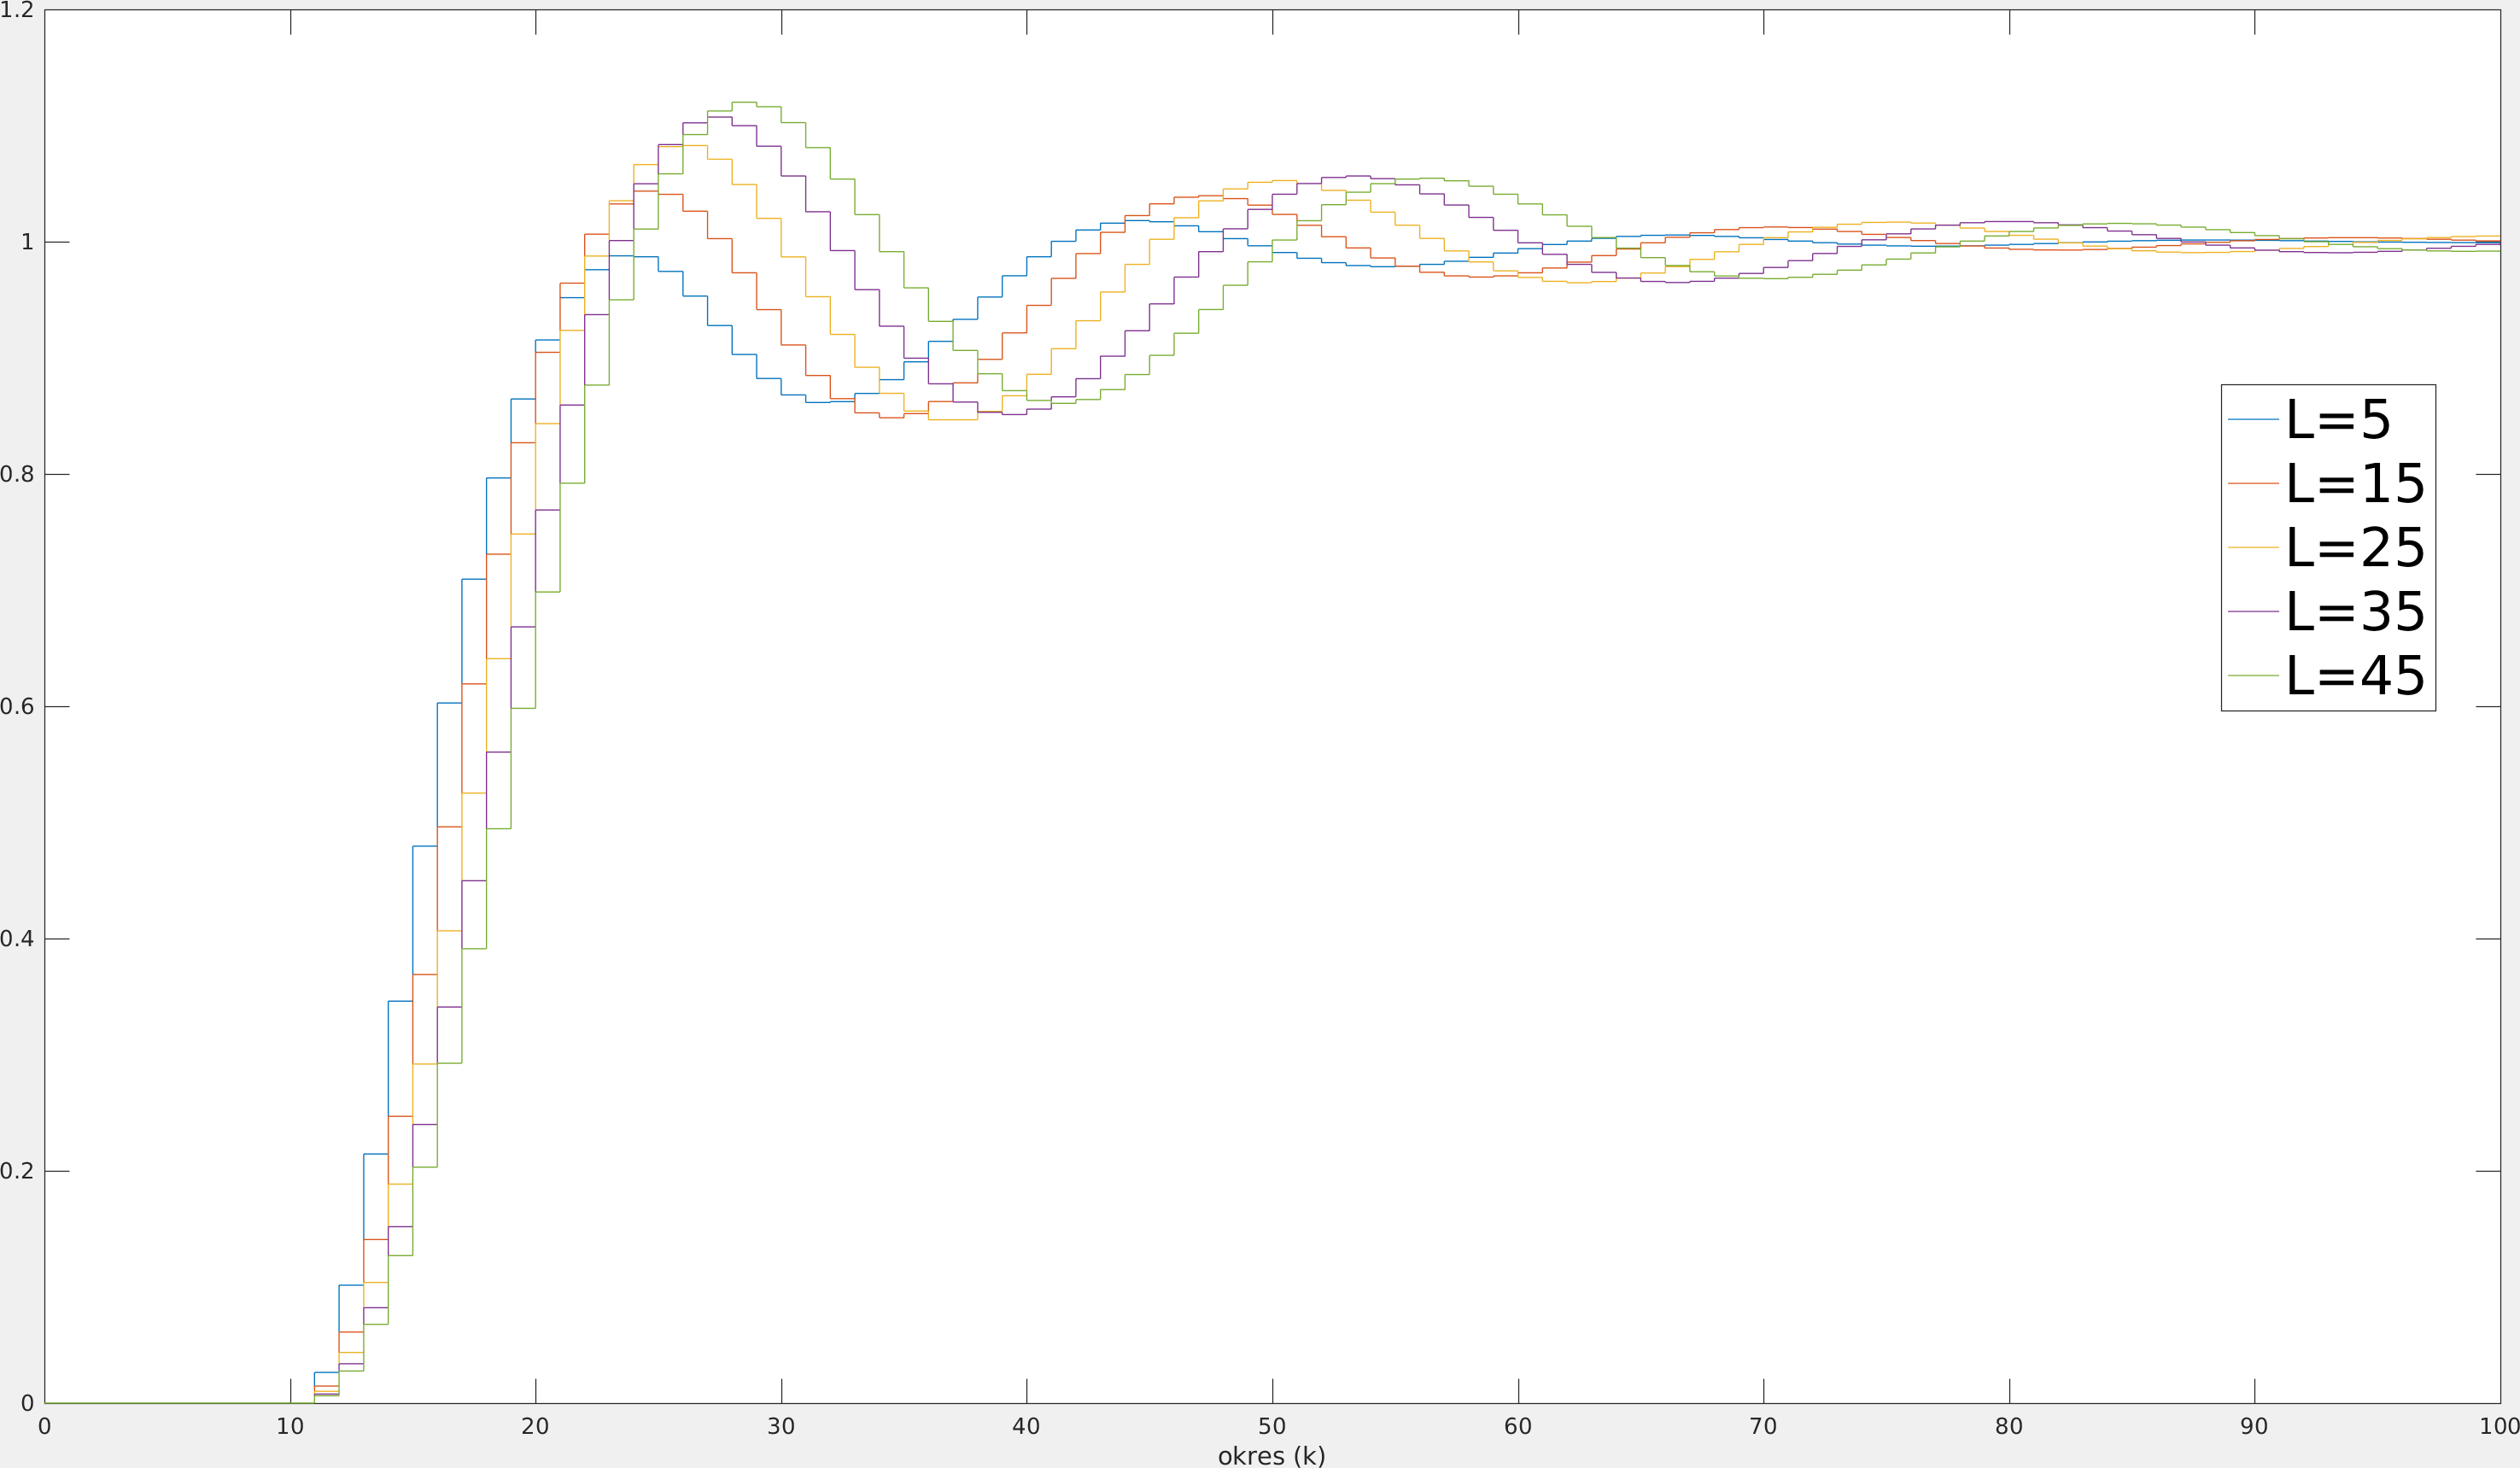
\includegraphics[width=\textwidth]{scripts/zadanie5dwyjscie2.png}
		\caption{wyjście obiektu regulacji dla kolejnych wartości parametru $\lambda$}
	\end{figure}
	\begin{figure}[H]
		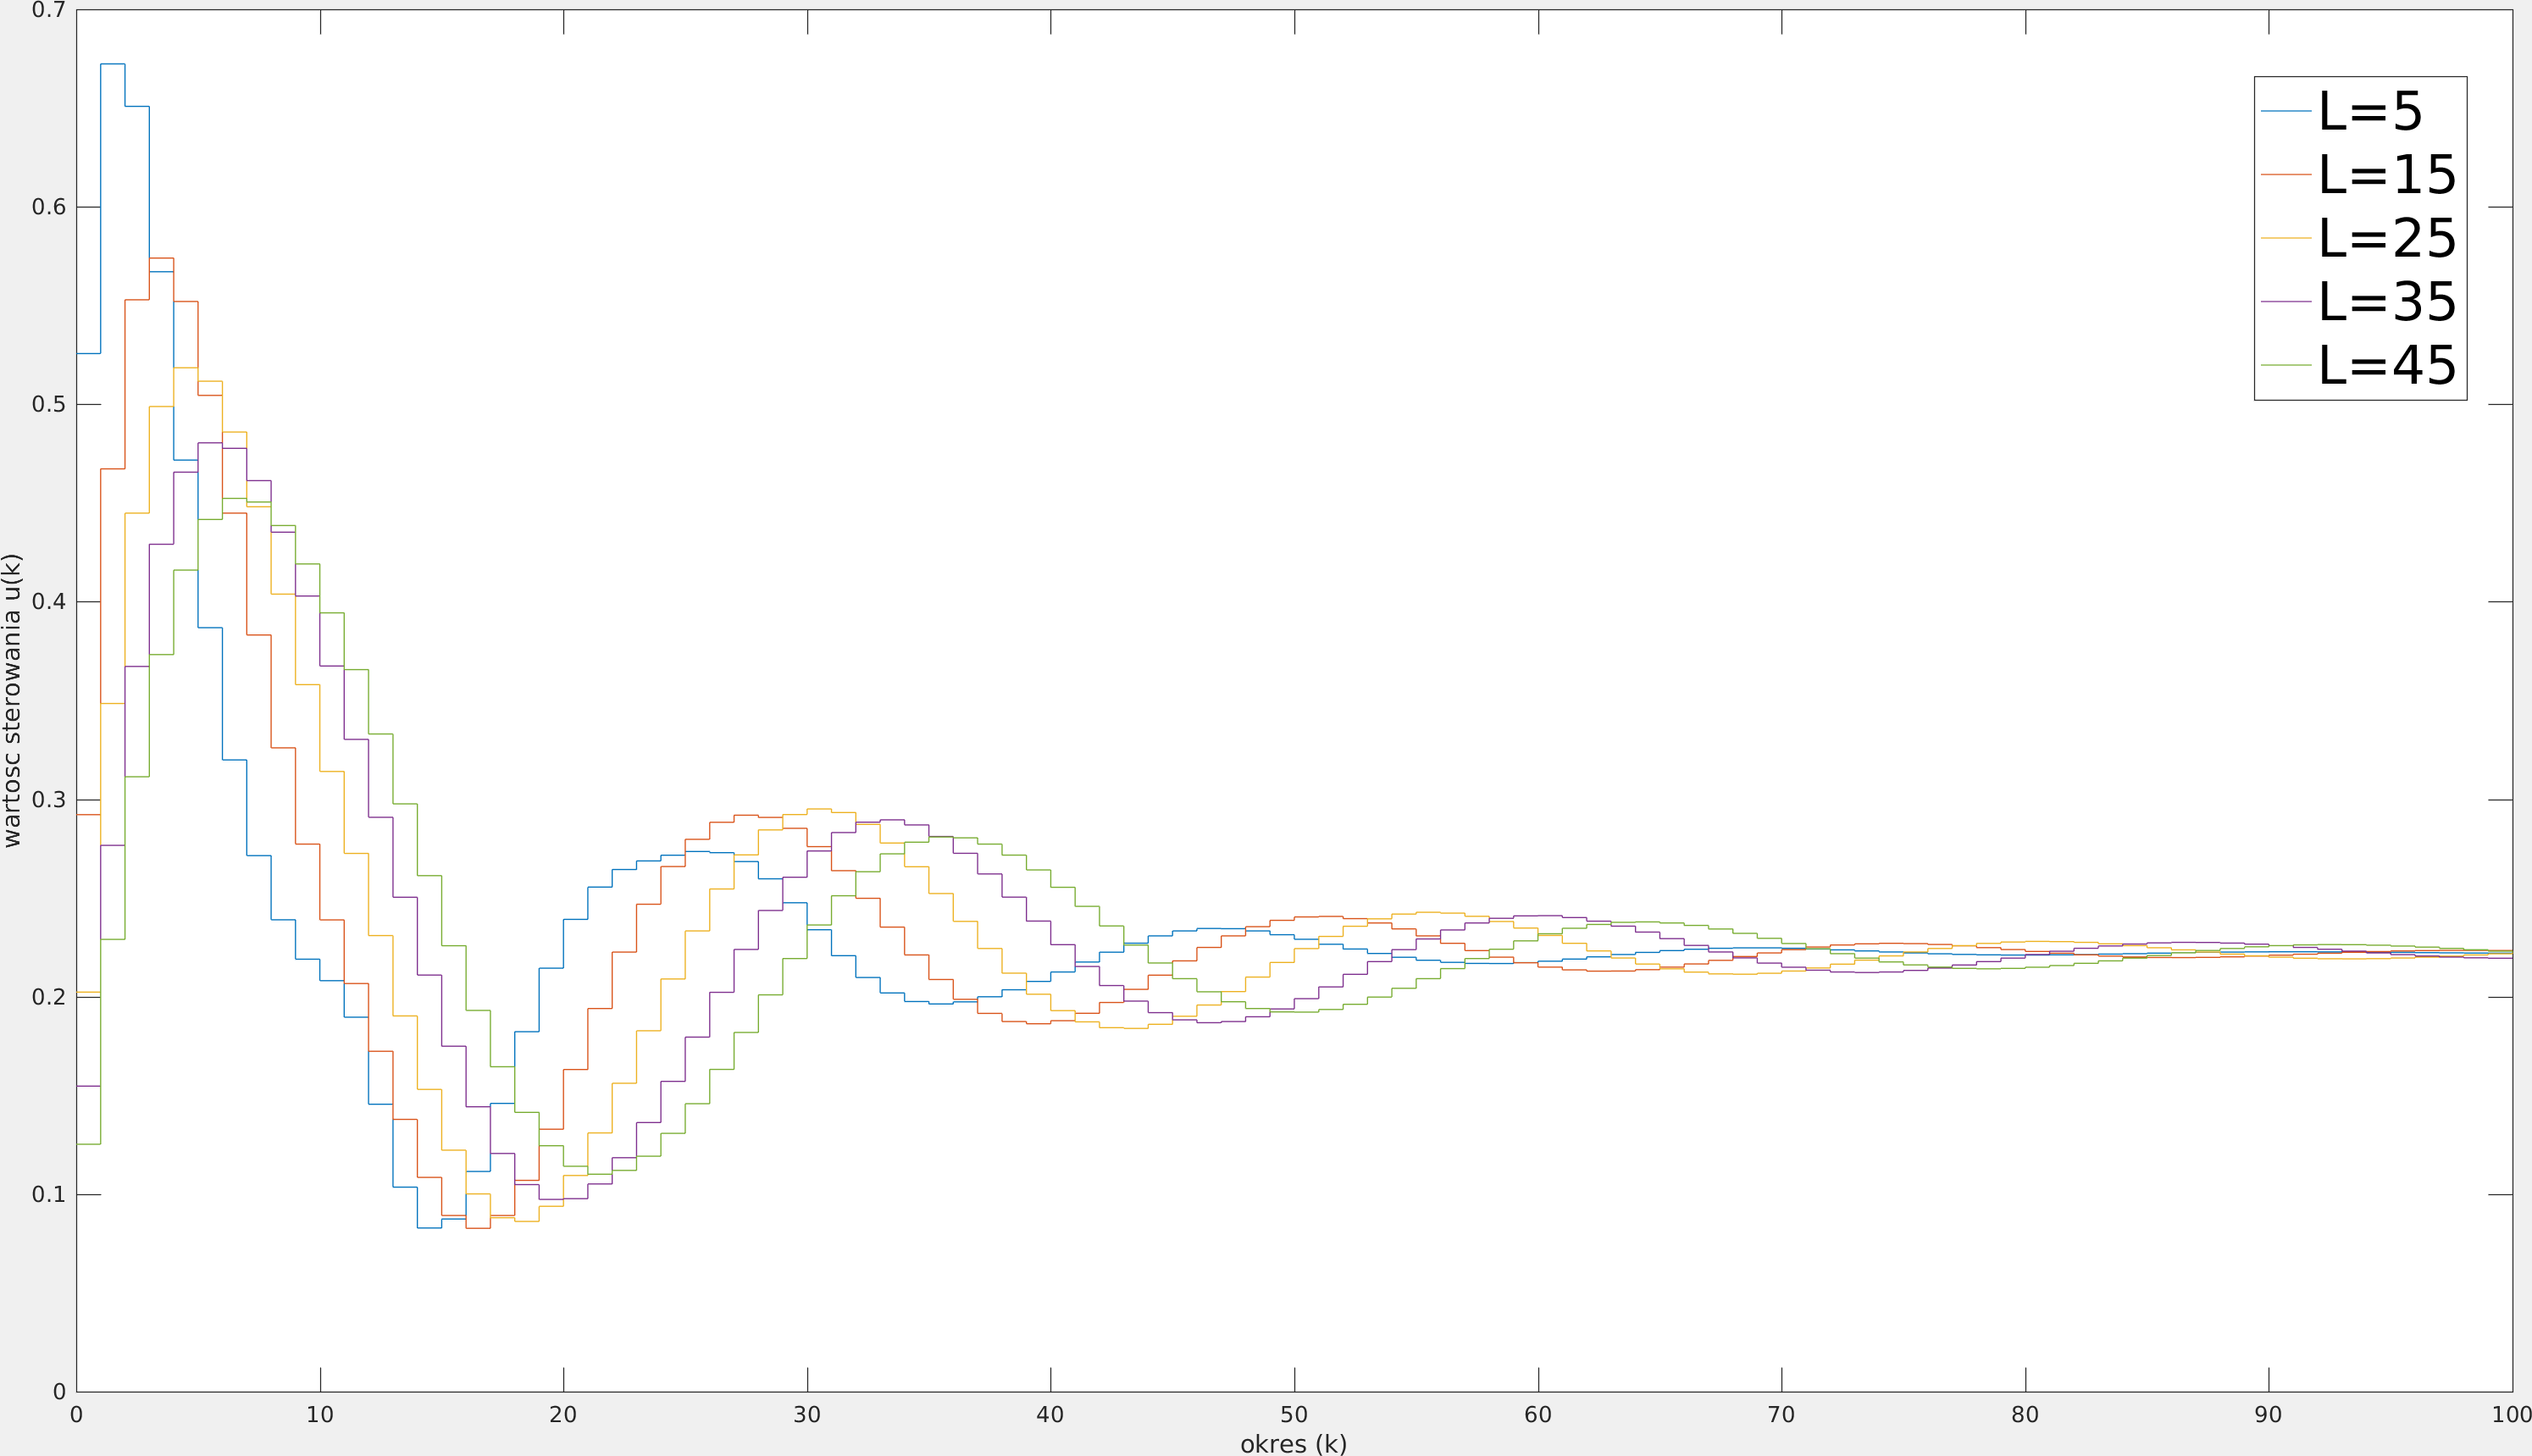
\includegraphics[width=\textwidth]{scripts/zadanie5dster2.png}
		\caption{wartość sterowania obiektu regulacji dla kolejnych wartości parametru $\lambda$}
	\end{figure}

	Zwiększanie wartości parametru $\lambda$ zwiększa czas regulacji, ale zdecydowanie zmniejsza wartości sygnału sterującego. Dla wartości $15$ daje podobną odpowiedź obiektu jak w przypadku dłuższego horyzontu sterowania w poprzednim punkcie, ale zdecydowanie zmniejsza wartości sterowania, dlatego zdecydowano się wybrać właśnie tą wielkość.

	\section{Obszary stabilności}

Ostatnim zadaniem było wyznaczenie maksymalnych zmian obiektu, po których regulacja danym regulatorem nie była by możliwa, a następnie zdecydowanie, który algorytm jest bardziej odporny na zmiany obiektu. Przeprowadzono symulacje zmian wartości $T_o$ oraz $K_o$ tak aby uzyskać funkcję granicy stabilności $K_o/K_o^{nom}(T_o/T_o^{nom})$, gdzie $T_o/T_o^{nom}$ zawiera się w wartościach ${1.1;1.2;1.3;1.4;1.5;1.6;1.7;1.8;1.9;2}$.

Proces przeprowadzania eksperymentu dla każdego z poniższych regulatorów był tożsamy - najpierw ustawiano wartość opóźnienia obiektu $T_o$ tak, aby był spełniony stosunek podany w wymaganiach zadania. Zaczęto od wartości $T_o/T_o^{nom}=1.1$. Następnie sukcesywnie zwiększano wartość $K_o$ aby dotrzeć do granicy stabilności obiektu. Po ustaleniu granicznej wartości następowało przejście do następniej wartości $T_o/T_o^{nom}$ i rozpoczynano proces od początku.

Poniżej znajduje się wykres wartości granic stabilności dla regulatorów PID z nastawami Z-N, poprawionymi oraz algorytmu DMC z wyznaczonymi w poprzednim punkcie parametrami $D, N$ oraz $N_u$ i $\lambda$.

\begin{figure}[H]
	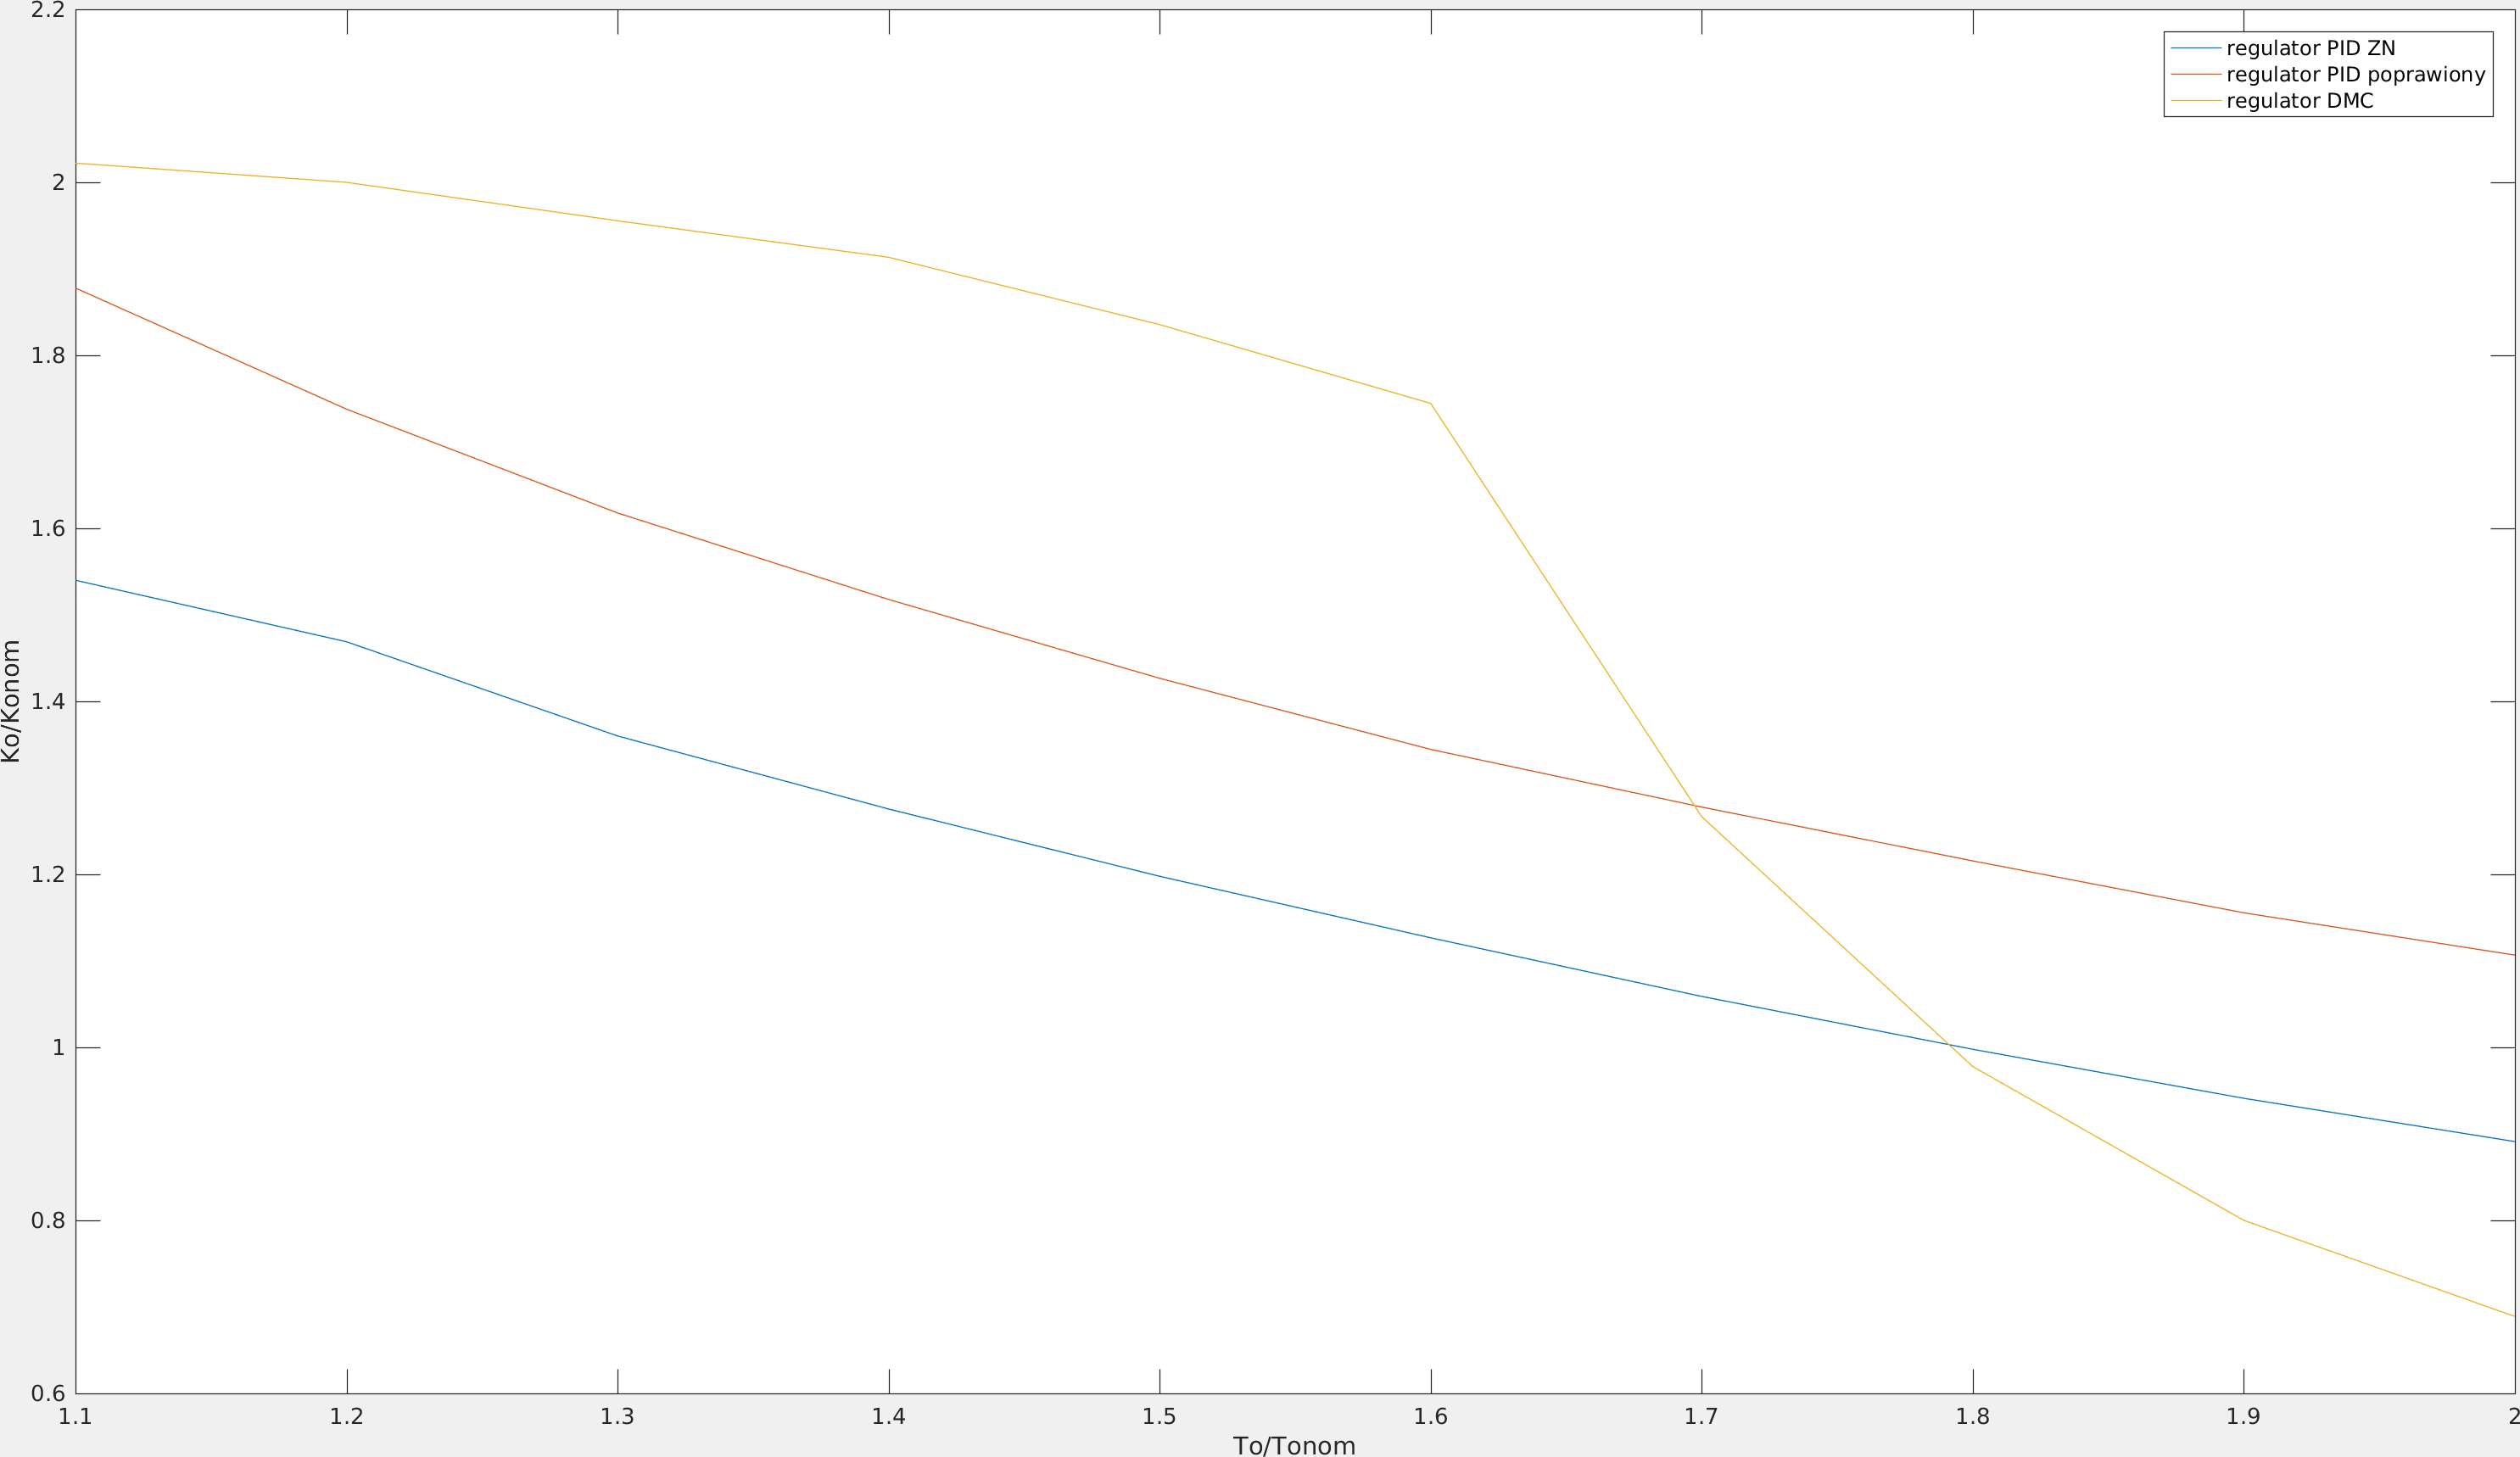
\includegraphics[width=\textwidth]{scripts/zad62.png}
	\caption{granice stabilności dla algorytmów PID oraz DMC}
\end{figure}

Pierwszą rzeczą, jaka jest widoczna od początku, jest przewaga zapasów stabilności regulatora DMC nad regulatorem PID. Chociaż dla dobrze dostrojonego algorytmu proporcjonalno-całjąco-różniczkującego na początku ta różnica nie jest duża, to w połowie testu zapasy DMC zaczynają gwałtownie maleć, więc różnica między algorytmami szybko topnieje i zamieniają się miejscami. Można wysnuć wniosek, że algorytm DMC jest bardziej odporny na mniejsze zmiany opóźnienia obiektu

Warto również zaznaczyć, że lepiej dostrojony algorytm PID ma większe zapasy stabilności niż ten z nastawami Z-N, mimo że te prawie liniowo wciąż się zmniejszają.

\section{Podsumowanie}

Porównując obydwa algorytmy można stwierdzić, że regulator DMC ma więcej zalet. Jest nieco trudniejszy do implementacji, lecz powoduje zdecydowanie krótszą regulację, jest łatwiejszy do dostrojenia i ma większe zapasy stabilności, dopóki nie przekroczy się granicy horyzontu predykcji.

Za to regulator PID jest prostszy w implementacji, nie ucina nagle procesu regulacji dla zbyt dużych zmian obiektu i początkowo niewiele odstaje zapasami stabilności od algorytmu DMC. Jego regulacja jest jednak dużo bardziej skomplikowana.

Można więc stwierdzić, że do obiektów z opóźnieniem oba algorytmy znajdą swoje zastosowanie, lecz algorytm DMC jest bardziej użyteczny i przyjazny.


\end{document}
